\RequirePackage[hyphens]{url}
\documentclass[11pt,3p,twocolumn]{JMN}

\usepackage{amsmath}
\usepackage{amsfonts}

\usepackage{totpages}
\usepackage{ragged2e}
\usepackage{color,pxfonts}
\usepackage{latexsym}
\usepackage[mathletters]{ucs}
\DeclareUnicodeCharacter{32}{$\ $}
\usepackage[T1]{fontenc}
\usepackage[utf8x]{inputenc}
\usepackage{pict2e}
\usepackage{wasysym}
\usepackage[english]{babel}
\usepackage{tikz}
%\usepackage{authblk}
\usepackage{graphicx}
\usepackage{geometry}
\usepackage{times}
\usepackage[norule,symbol,perpage]{footmisc}
\usepackage{fancyhdr}

\usepackage{wrapfig}
\usepackage{epsfig}
%%\usepackage[hidelinks,colorlinks=true,linkcolor=blue,citecolor=blue]{hyperref}
\usepackage{natbib}
\bibliographystyle{agsm} %Harvard Bibliography style
%%\usepackage{hyperref}
\usepackage{cleveref}

\biboptions{authoryear,sort&compress}
\setlength{\bibhang}{0pt}

\setlength{\headheight}{15pt}
\renewcommand{\headrulewidth}{0pt}
\renewcommand\harvardurl[1]{\textbf{URL:} \url{#1}}

% For Single column
%\setlength{\textwidth}{40pc}
%\hoffset=-1cm
%\textheight=22.5cm

% For two column
\setlength{\textwidth}{38pc}
\hoffset=-1cm
\voffset=-0.5in
\textheight=23cm
\setlength\parindent{0pt}

% Keywords command
\providecommand{\keywords}[1]
{
  \small	
  \textbf{\textit{Keywords---}} #1
}

\begin{document}

\pagestyle{fancy}
\fancyhf{}
\lfoot{Volume X, Issue Y, ZZZZ}
\rfoot{\thepage}

\begin{frontmatter}

\title{The evolution of GENESIS: From simulation to emulation neuroscience}

\author[a,1]{Hugo CORNELIS} 
\author[b]{Allan D. COOP} 

\address[a]{\noindent Neurospaces Development, Daniëlstraat 27, 3500 Hasselt, BELGIUM}

\address[b]{Three Way Street, PO Box 140, Grenfell, 2801 NSW, AUSTRALIA\vspace{0.5cm}}

\address[1]{Corresponding author: {\bf hugo.cornelis@google.com}}

\begin{abstract}
The history of computational neuroscience reveals that the extension of simulator functionality typically results in the unintentional creation of monolithic software platforms.  A major source of the difficulties involved with simulator extensibility faced by many software developers emerges from the role played by their primary focus on the cognitive models of organisational structure assumed for nervous systems. As an alternative, here it is proposed that the problems currently encountered when interpreting the mammalian nervous system arose during the Classical and pre-Classical eras and continued to further reveal themselves following refinement during the Enlightenment. This has been compounded by assumptions concerning the mathematical implementation of a model and its underlying software architecture, at the expense of considering biological structure and function. This greatly increases the difficulty of extending simulator software code to support the new functionality required by efficient scale-independent simulations.  It limits software development efforts, thus simulator functionality, and ultimately simulator extensibility. Here, axioms are proposed that define the domain of simulation neuroscience. They have been extracted from over twenty years of simulator and model development by the global GENESIS developer community and provide a logical framework that organises the approach to scale-independent simulation that is introduced here. This framework, referred to as the CBI federated software architecture, underpins the reconfigured GENESIS simulator.  The outcome is resolution of the many problems associated with multiscale modelling that previously existed when a simulator incrementally transformed into an unmanageable monolith. Careful consideration of the issues identified has greatly facilitated the development of a simulator competent to transparently support biological models in a scale-independent manner across resolutions ranging from the ionic and molecular to completely integrated systems.
%%The approach to development of simulator structure and function is outlined by describing essential components of the CBI federated software architecture for scale-independent modeling.
\end{abstract}

\begin{keyword}
list your keywords here, e.g.  keyword1, keyword2, keyword3, keyword4, keyword5, etc

\vspace*{1\baselineskip}
\hspace*{0.05\textwidth}\begin{minipage}{0.9\textwidth}

\noindent ``\small{\textit{That \textnormal{[a]} model is not true is certainly correct, no models are—not even the Newtonian laws. When you construct a model you leave out all the details which you, with all the knowledge at your disposal, consider inessential \ldots. \textbf{Models should not be true but it is important that they are applicable}, and whether they are applicable for any given purpose must of course be investigated. This also means that a model is never accepted finally, \textnormal{[it is always]} only on trial}.}''\\
---\citet[pp.\,37--38]{rasch80}.\\
\end{minipage}

\end{keyword}

\end{frontmatter}

%\vspace*{-1\baselineskip}

\vspace*{-8\baselineskip}
\definecolor{color_197966}{rgb}{0.686275,0,0}
\begin{tikzpicture}[overlay]\path(0pt,0pt);\end{tikzpicture}
\begin{picture}(0,0)(70,-520)
\put(-10,-845.4799){
\includegraphics[width=47.64pt,height=875pt]{JMN_image.png}}
\put(67,-20.0){\fontsize{14.04052}{1}\usefont{T1}{cmr}{b}{n}\selectfont\color{color_197966}Perspective}%% Original Research/Review/Perspective}
%%\put(67,-43.23993){\fontsize{14.04052}{1}\usefont{T1}{cmr}{b}{n}\selectfont\color{color_197966}Perspective}%% Original Research/Review/Perspective}
\put(490.76,-25.0){
\includegraphics[width=38.28pt,height=38.28pt]{Neuralpress_image1.png}}
%%\put(490.76,-59.36){
\includegraphics[width=38.28pt,height=38.28pt]{Neuralpress_image1.png}}
\end{picture}

\vspace*{3.2\baselineskip}
%\twocolumn

\section{Introduction}

The structure, components, and functionality of multicellular organisms are inherently complex~\citep{walpole13}. However, it has been shown for a variety of different nervous systems and the human central nervous system in particular, that they operate across diverse internal domains to sustain development, growth, and reproductive potential~\citep[see for example][]{selverston87,vonk22,kandel21}. Such activity extends from the most basic amino acid substitutions that alter protein function to concerted multicellular signalling cascades that regulate hormone releases thereby modulating behaviours throughout an entire lifecycle. Scientific research into these domains has led to precise computational models that have been valuable products of the current human understanding of neurobiology~\cite[see for example][]{bower13,nandi22}. These realistic models capture aspects of component function and interactivity within the neurophysiological expanse assumed to exist between isolated {\it{in\,vitro}} experiment and whole-organism behavior.
One software platform that has successfully been employed to implement some of these realistic computational models is the GEneral NEural SImulator System~\citep{bower03}.

With a history of over 35 years, a recent reconfiguration of the GENESIS platform for realistic modelling of neural structure and function has brought to an end what in hindsight can now be referred to as the classical period of computational and simulation neuroscience.

Consequently, a primary aim here is to briefly explore and describe the major philosophical and computational frameworks that underlie this recent software reconfiguration from which GENESIS 3.0 (G-3) has emerged. In this reconfiguration the the historical monolithic core of GENESIS has been completely restructured and reimplemented as a system of independent software components. Based on the modular CBI architecture~\citep{cornelis12}, G-3 now consists of a set of largely independent components which can be used either individually or in combination to perform the functions desired in running a given simulation. Keeping with the original design objectives for the GENESIS project, this modularization considerably enhances the ability to run models across different levels of biological scale, and greatly facilitates interactions between those levels.

In doing so, significant moments in the evolution of the classical paradigm established for neuroscience generally and computational and simulation neuroscience in particular, are briefly revisited. Subsequently, a conceptual framework is briefly elaborated. This framework, which accounts for both conceptual models and their computational implementation, is proposed to provide a principled foundation for the next phase of research in the theoretical neurosciences. Further, it is expected to inspire considerably more creative and realistic approaches through the generation of new models and procedures, collectively referred to as emulation neuroscience.

A reconfigured paradigm is predicted to lead to the evolution of a considerably more sophisticated scientific understanding of the central nervous system, thus contribute to further resolution of the highly challenging problems that continue to confront active neuroscientific research. To paraphrase Immanuel~\citeauthor{kant08} (1755, republished~\citeyear{kant08}), the foregoing is a subject which, in view of its inherent difficulty, can at the outset elicit unfavourable judgment from a large proportion of readers; as initially was the case for {\it The Structure of Scientific Revolutions}~\citep[][see also~\citeauthor{mahfoud21}~\citeyear{mahfoud21}]{bird22}.

% To this end, the most widely accepted historically inherited schema, modified, and elaborated during the last 40 years is briefly revisited. This is followed by several brief examples that assist with moving from the paradigm of classical neuroscience to one that gives a more accurate dynamic conceptual model of the structure and function of the human brain, that is proposed to enable more realistic simulation of neurophysiological function and its consequences. The aim is to better align historically driven cognitive models of mammalian brain structure and function with historical observations and contemporary empirical reports.

% After introducing a perspective for the current paradigm by which contemporary neuroscience generally and computational neuroscience in particular have evolved, the reconfigured GENESIS 3.0 simulation platform arrived at through the CBI federated software architecture is introduced and briefly described.

\begin{figure*}[h!t]
  \begin{center}
    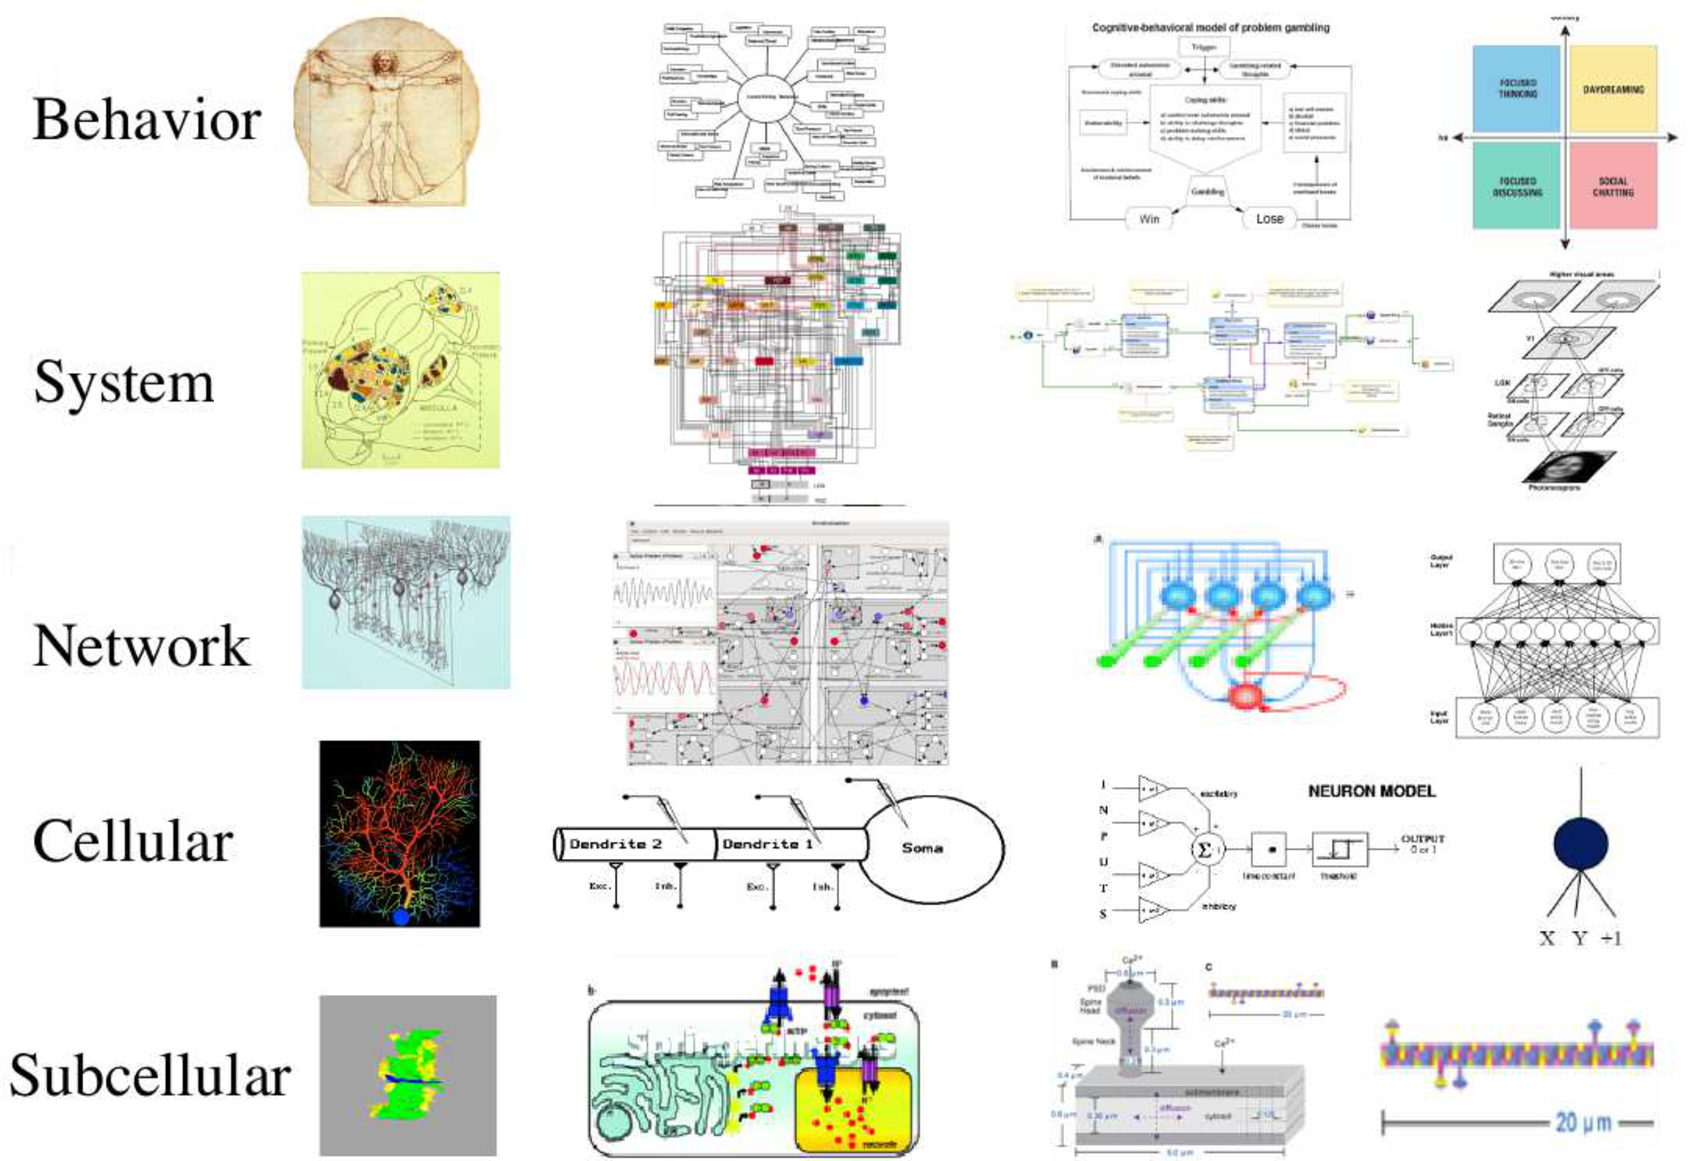
\includegraphics[width=0.9\textwidth]{figures/multi-scale-taxonomy-no-arrows-no-texts.pdf}
    \caption{ \small{\bf A model taxonomy.} }
  \end{center}
  \label{fig:multi-scale-taxonomy}
\end{figure*}

\subsection{Evolution of the Classical Neuroscientific View}

Previously described as an "enchanted loom"~\citep{sherrington53}, the central nervous system can be seen as an orchestrated constellation of cellular webs. Alternatively, engulfed by the mechanical age~\citep{carlyle52}, ~\citet{meyers87} proposed to his readers to imagine the human brain as a vast manufactory, in which thousands of looms, of complex and differing patterns, are habitually at work, a claim likely inspired by the mechanical world views of ~\citet{descartes62} and before him ~\citet[][republished 2003]{fernel67}. 

Subsequently, almost one hundred years after Meyers, one of the earliest practical schemes developed to provide a framework for computational modelling of neurophysiology was that developed by~\citet{Marr:1982fk}. He identified three independent levels for understanding visual processing: (1) Computational theory---What is the goal of the computation, why is it appropriate, and what is the logical strategy by which it can be achieved? (2) Data and algorithm---How can a given computational theory be implemented? In particular, what is the structure and content of inputs and outputs and what is the algorithm for their transformation? (3) Hardware implementation---How can structure, content, and algorithm be physically realized?

An important element of this view was that higher level questions came to be considered largely independent of lower levels. Thus, analysis at the highest level, i.e. Level (1), was independent of any understanding of the algorithm(s) that supported a given computation at Level (3). Similarly, analysis at the intermediate Level (2) required no understanding concerning its physical implementation. 

\subsection{Current Status of Computational Neuroscience}

Figure~\ref{fig:multi-scale-taxonomy} illustrates a representative example of the current status of computational neuroscience. In this figure, the column to the left gives a set of labels that each define a biological level (Behavior, System, Network, Cellular, Subcellular) at which a given computational model is typically implemented. The next column provides a pictorial illustration typical for each of the given levels. The remaining three images associated with each level expand the abstraction of the initial pictorial illustration. When combined, the illustrations and abstractions generate a matrix that respectively characterize one possible taxonomy of a set of conceptual and computational models.

Figure~\ref{fig:multi-scale-taxonomy} also captures that individual modeling projects within one or more laboratories typically tend to focus on the implementation and study of a single model at a given level. This tendency acts to both isolate each research program and creates the problem of how to integrate resultant but effectively independent models. This problem is only exacerbated as new empirical data is acquired at any level of biological detail, a problem that can be referred to as the monolithic problem. This occurs when continual modification and/or expansion of a software platform results in a coding syestem that becomes increasingly unmanagable. In short, Figure~\ref{fig:multi-scale-taxonomy} provides a graphic illustration of what has come to be known in computational neuroscience as the multiscale problem.

Here, it is proposed that problems, such as the unintentional creation of monolithic software as computational models and simulations have become engorged by increasing scale and complexity and consequently an increasingly befuddle computational and simulation neuroscience, can be attributed to the confluence of several foundational factors. They include the increased effect of historical assumptions that evolved from Platonic and Aristotelian philosophy that, following neo-Platonic refinement through the Medieval Period, by the time of the Elizabethan Period had developed into an increasing and profoundly culturally entrenched metaphysics. This process structured subsequent theological beliefs that then became subsumed into the rapid expansion of science during the Enlightenment to became foundational beliefs driving cognitive understanding and organization of the developing biological sciences following the Enlightenment. Subsequently, these theological beliefs and metaphysical assumptions came to form the central dogmas of the neurosciences and particularly the theoretical and mathematical implementations that were chosen to match the computational and simulation neurosciences. In short, a theological Celestial Hierarchy that defined humanity's relation to God was subsumed into a Great Chain of Being that ordered and described the levels, attributes and hence roles of life in a hierarchy that spanned a possibly infinite range of levels from the non-living to humanity and beyond through realms of angels and ultimately, God. Thus, a hierarchical framework originating in a theological world view has come to provide an unquestioned organizational paradigm for an understanding of the structure of the mammalian central nervous system, a sequence of events and it implications for theoretical and mathematical neuroscience and its implementations that is further explored below in the Discussion.

In contradistinction to these foregoing core beliefs of the biological sciences, and their problematic nature, an alternative is proposed here that already has begun to resolve significant aspects of the problems of monolithic software code and multiscale modelling currently faced by computational and simulation neuroscience. Based on the notion of heterarchy, it provides the basis of a world view where cause and effect are replaced by change and consequence.

\subsection{Refining the Classical Approach}

More recently, with reference to~\citet{Marr:1982fk},~\citet[][C\&S]{Churchland:1992uq} proposed a refined version of his three level schema: (1) Level of analysis, which includes Marr’s three levels, (2) Level of processing, for example the levels of processing in the visual pathway, and (3) Level of structural organization, for which they proposed seven general levels (Systems, Topographic Maps, Layers and Columns, Local Networks, Neurons, Synapses, Molecules). In developing their perspective, a number of fundamental observations were made.

Importantly, it was noted that the doctrine of independence confuses two very different issues. One concerns whether as a matter of discovery the relevant algorithm can be determined, while the other concerns whether as a matter of formal theory, a given algorithm already known to perform a task on a given machine (in this case, the brain) can be implemented on a machine with a different architecture. Computation theory suggests that if an algorithm is independent of its implementation it can also be implemented on different machines with different architectures as none of the requisite physical parameters are part of the algorithm. In short, there is no formal theory to confirm whether the discovery of the algorithms relative to cognitive function are independent of the detailed structure of the nervous system.

In contrast to the doctrine of independence, current research suggests that implementational considerations play a vital role in the kinds of algorithms that tend to be devised and the types of computational insights that they provide (C\&S); whereas, knowledge of brain architecture, far from being irrelevant as proposed by the top-down modellers, may provide an essential basis for likely and powerful algorithms.

Finally, in brief, whether unintentional or not, C\&S's position appears to be a clear restatement of the secular interpretation of {\it{The Great Chain of Being}}. The framework developed by C\&S, can be seen as an example {\it{par excellence}} of a simplification of cerebral cytoarchitecture that that reinforces a long-standing organizational framework that appears to continue to provide the predominant understanding of the principles of neural structure and function in the mammalian central nervous system. One that remains embedded in philosophical framework composed of hierarchical levels of organization and function. It is a paradigm that necessarily continues to predetermine much ongoing theory and many ideas considered fundamental to increased understanding of mammalian nervous systems in general and particularly their central nervous systems.

\subsection{Collapse of the Classical Approach}

One of the most surprising statements associated with the emergence of computational neuroscience was made by C\&S. As suggested by Figure~\ref{fig:multi-scale-taxonomy}, they postulated the primacy of levels as a foundation of the computationally modern view of the neurobiological research paradigm. Given the historical considerations introduced above, such a dogmatic stance appears to be a reactionary curiosity, even when initially proposed. An important question then becomes, how did such an assumption come to be so central to understanding the neural structures and functions that subserve neurophysiology?

C\&S's position on levels is a simplifying statement that greatly increases the tractability of gaining better understanding of the mammalian central nervous system. This is despite going against powerful observational and theoretical evidence that seems to support a novel emerging understanding of the highly dynamic structure and function of the human brain. This perspective starts at least with observations made by anatomists such as~\citet{bell11}. More than 200 years ago, he noted that in the lack of any consistent history of the brain and nerves, along with the dull unmeaning manner of demonstrating the brain, any novelty in the manner of treating the subject was authorised. Further, that it is no more presumptuous to follow the tracts of nervous matter in the brain and attempt to discover the course of sensations, than it is to trace the rays of light through the humours of the eye and to say that the retina is the seat of vision. Things appear sufficiently simple and consistent until the structure of the brain and the course of the nerves are begun to be examined anatomically. Then all is confusion. The divisions and subdivisions of the brain, the circuitous course of nerves, their intricate connections, their separation and reunion, are puzzling in the last degree and are indeed considered as things inscrutable. Thus, those who know the parts the best are the most in a maze. While, those who know the least anatomy, see the least inconsistency in the commonly received opinion.

%%Comments such as those made by~\citet{bell11} are supported by observations made more than 250 years previously by Fernel and followed a century later by Descartes who (as quoted by \citeauthor{sherrington53}~\citeyear{sherrington53} was putatively following Fernel) is considered to have originated the view that living organisms worked as machines and insisted on a class of motor acts, animal and human, in which the thinking soul takes little or no part~\citep{descartes62}.
By the middle of the twentieth century it could be said that the classical viewpoint was finally beginning to be upended by theoretical publications such as that authored by~\citet{mcculloch45}. Entitled, {\it{A heterarchy of values determined by the topology of nervous nets}}, it proposed that because of both the reciprocal nature of purposive activity and the closed circuits sustaining it and their interaction, the circuits can be treated topologically. If it is recognised that {\it{A}} is preferable to {\it{B}}, {\it{B}} to {\it{C}}, but {\it{C}} is preferred to {\it{A}}, there is a  corresponding circularity in the net that is not the path of any one circuit and cannot be mapped. He concludes that an organism possessed of such a nervous system---six neurons--- is sufficiently endowed to be unpredictable from any theory founded on a scale of values. It lacks a hierarchy of values and instead exhibits a heterarchy of values and thus its connectivity is too rich to submit to a {\it{summum bonum}}.

\subsection{Collapse of the Computational Approach}

GENESIS (the GEneral NEural SImulation System) was one of the first general purpose open source software platforms designed to support the simulation of neural systems ranging from subcellular components to system-level models (see http://genesis-sim.org). It first became available in 1988, with a full public release in 1990, followed in 1995 by GENESIS version 2.0~\citep{jung22}. In 2014 the final packaged version of GENESIS (version 2.4) was released with any further community development made available from the Repository for Continued Development of the GENESIS 2.4 Neural Simulator (https://github.com/genesis-sim/genesis-2.4).

The innovative beginnings of the GENESIS software simulation platform were based on a number of assumptions with regard to the aims of computational neuroscience. These assumptions included, amongst others: (1) The construction of ``realistic" computer models based on actual anatomy and physiology is an essential prerequisite for understanding the computational organization of the nervous system, (2) Understanding nervous system function depends upon being able to construct and link models at many different levels of biological scale, (3) Growth of a modeling system is reliant on the ability of individual modelers to develop and share model features and components, (4) The system should be as machine independent as possible, and (5) Successful use depends on a graphical interface that supports users with different ranges of computer expertise.

More than a decade prior to the release of GENESIS 2.4, it was realized that rather than just component modularity, what was required for a simulation package in computational neuroscience was a collaborative system~\citep{cornelis03}. In such a system a small extensible core or kernel manages a set of modules and components that engage in shared activities via semantically defined interfaces. In the absence of such a software architecture even the most valiant coding efforts in computational neuroscience were found to ultimately result in what might be referred to as a monolithic software architecture. In such an architecture it is difficult to extend a simulation platform and it becomes increasingly difficult to construct and simulate complex neuronal models even when their size and complexity is only incrementally increased.

It was found that a major reason forcing the evolution of a software platform into a monolithic architecture occurs when the data model employed is insufficient to account for all the requirements of a realistic model. Typically, this occurs when the mathematical implementation of a model looses its conceptual dimension. This puts pressure on the cognitive model developed by an investigator. It results from the fact that they are forced to think about the computational model in a mathematical way as it is actually instantiated by code that not only constructs all required neural populations but also the links necessary for the network connectivity of individual neurons.

In more detail, the problems of a monolithic software architecture emerge as the hierarchical function and three-dimensional nature of a complex cognitive model is incorporated into ever-larger computational simulations. Following the model setup phase, both the topology of the network and the projections between the various populations typically are lost. This occurs when the projections and connections of individual neurons exist within and between different levels of the network hierarchy, yet all connections require inspection at each stimulation timestep. Ultimately, this is a problem that is only exacerbated as neuronal populations are enlarged, whereby each constituent neuron becomes both source and target for increasing connectivity.

\subsection{Borrowing From the Physical Sciences May Not Help}

Currently, there are no published data models in computational neuroscience sufficient to resolve the foregoing problems and the resultant models typically exist as flat two-dimensional networks, not as realistic three dimensionally structured simulations. This dilemma is only further compounded by the requirements of modelling that aim to incorporate increasingly realistic detail into a simulation, such as conductance scaling and compound models of heterogeneous intracellular mechanisms. Attempts to circumvent these problems by, for example, integrating existing software packages into a collaborative system~\citep{goddard01:_neosim} or by making mathematical libraries accessible as object-oriented class hierarchies~\citep{vibert01} have proved unsuccessful~\citep{cornelis03}.

Alternatively, agent-based modeling and cellular automata have successfully been employed to model aspects of the mammalian immune system~\citep{chiacchio14}. Such bottom-up models belong to a class of discrete mathematical approaches in which entities (agents) sense local information and undertake actions over time according to predefined rules. Interactions are described and followed individually, with the general behavior of the system arising from the sum of the local behaviors of the involved entities. This allows local processes to be described more accurately by avoiding the rough approximations typical associated with top-down approaches. Their strength is characterized by the appearance of a global behavior that emerges from interactions among agents. However, as it does not follow linear rules and is often stochastic by design, model behavior can be quite unpredictable,. This requires in turn the adoption of Monte-Carlo simulation methods to determine the statistical behavior typical of simulations. With the assistance of a multiscale platform, the response of CD4+ T cells to infections has successfully been explored~\citep{wertheim21}. In that case, at the highest level the simulation algorithm employed agents in a series of fixed time steps, the number and size of which were determined by the duration and resolution of the modeled event, respectively. Simulations based on such an approach rely on strong mathematical theory that in some cases allows analytical study and asymptotic analysis. However, simulating the complex systems subserving cognition and behavior found in the mammalian nervous system ultimately reveals intractable problems, such as those associated with the implementation of multilevel simulation and the monolithic simulators that as a consequence inevitably seem to appear.

Somewhat prior to the agent-based approach, a bottom-up approach was developed that, starting from the molecular level, consisted of the integration of molecular events into synaptic and neuronal architectures~\citep{bouteiller11}. It showed that small modifications of critical parameters at a molecular resolution may have significant impact at a neuronal resolution. Such studies support the proposition that mathematical theory and associated algorithms suited to multiscale simulation in the physical sciences may not be entirely appropriate for exploration and development of an understanding of the complexity and functions of neurobiological structure.

A further example of the conceptual implementation problems that arise from the still prevalent classical cognitive frameworks introduced by Marr and C\&S, is that they only appear to be resolved by plausible approximation. In the spirit of Marr's doctrine of independence, a recent review~\citep{deco08} of the computational modelling of the ``dynamic brain," stated its central theme to be that the activity in populations of neurons can be understood by reducing the degrees of freedom from many to few, hence removing an otherwise seemingly intractable computational problem. The most striking feature of the review is the claim that, the activity of a large population of spiking neurons can be reduced to a distribution function describing their probabilistic evolution (i.e. a function that captures the likely distribution of neuronal states at a given time) and that this function can further be reduced to give a single variable quantification of the population activity, the mean firing rate~\citep{deco08}. To understand how neuronal activity unfolds on a spatially continuous cortical sheet, neural field models involve differential operators with both temporal and spatial terms. Finally, at the microscopic scale an entire array of spiking neurons is simulated to obtain its response to a sensory-evoked synaptic current. By comparing that response to a mesoscopic neural mass model, what is gained and lost by abstracting to a more tractable set of evolution equations can be determined. In short, the flow terms in the high level neural mass model contribute to the expression of aperiodic dynamics in addition to those of the stochastic inputs. This is not possible in the planar microscopic system because chaotic dynamics require at least three degrees of freedom. Thus, the dimension reduction afforded by the neural mass approximation is proposed to allow the introduction of more complex intrinsic dynamics, permitting dynamical chaos. Whilst additional dimensions could have been added to the microscopic neurons, this would add to an already significant computational burden.

The field modelling approach just outlined, is a product of the physical sciences. This brings to mind comments by \citet{shannon56} about a new idea at the time, referred to as ``Information Theory" and its associated terms such as ``entropy" and ``redundancy." He noted they had permeated into numerous research domains within a decade of the publication of his mathematical theory of communication~\citep{shannon48}. He further observed that: It will be all too easy for our somewhat artificial prosperity to collapse overnight when it is realized that the use of a few exciting words do not solve all our problems. Rather the establishment of their application is not a trivial matter of translating words to a new domain, but rather the slow tedious process of hypothesis and experimental verification.

The foregoing concerns are some among many that permeate classical neuroscience and that when taken collectively suggest a modest proposal. Simulations capable of evoking cognitive recognition, insight, and understanding of the principles subserving the empirical mechanisms and functions of the known components and structure of the neurobiology under investigation, must match the data generated by both top-down and bottom-up simulations computed by a single unique code sequence. In the absence of such verification, it is difficult to convincingly assert that the algorithms identified and implemented in the name of computational or simulation neuroscience can directly be associated with the fundamental principles and mechanisms they purport to scientifically emulate.

As a general introduction to the following three sections to help with the distinction between Computationl, Simulation, and Emulation Neuroscience, it is noted that \S\ref{subsection:compneuro} refers to any computer-implemented method for exploring the properties of mathematical models where analytic methods are not available to predict the behaviour or outcome of a real-world physical system. In \S\ref{subsection:simneuro} a simulation is defined to provide a system model by mimicking some conditions and operations that lead to a final result. Whereas, as described further in \S\ref{subsection:emuneuro}, an emulator recreates an environment that allows observation of the conditions and execution of the operations of the original system.

\subsection{Computational Neuroscience}
\label{subsection:compneuro}

Ever since~\citet{lapicque07} in 1907, but particularly ~\citet{mcculloch43}, who found that for any logical expression satisfying certain conditions, a net exists that behaves in the fashion the expression describes; mathematics and computational methods have played an important role in understanding the nervous system. In the case of neurons, the fundamental ``realistic'' modeling approach following~\citet{hodgkin52e} has been to represent the electrical properties of biological membranes using an equivalent circuit consisting of capacitors and resistors in parallel~\citep[more recently, see][]{bedard13}. Computational neuroscience (also known as theoretical or mathematical neuroscience) is a field within neuroscience that employs mathematical models, computer simulations, theoretical analysis, and cognitive abstractions of the brain to understand principles that organize and control the development, structure, physiology, and cognitive activity of the (typically mammalian or invertebrate~\cite[for example,][]{}) nervous system. It employs computer-based calculations to validate and solve mathematical models and is considered to be either an important domain in or congruent to theoretical neuroscience~\citep{trappenberg23}. Further, the term mathematical neuroscience is also used sometimes, to stress the quantitative nature of the field.

To understand how the brain functions, it is necessary to understand its architecture. Just trying to guess its governing principles by relying on contemporary engineering ideas has resulted in little progress. \citet*{Churchland:1992uq} consider it an unavoidable conclusion that there is no substitute for fabricating proposals on the basis of observing real nervous systems, their components, connectivity, and interactions. Further, they consider it is the characterization of levels that is of primary importance and this it is this paradigm that forms their understanding as it did for~\citet{Marr:1982fk}. The proposals they make are further elaborated by the claim that their tripartite division of computational neuroscience really corresponds to three types of question: 1. How does a given question decompose into parts? 2. What principles govern how the parts interact in a given case? 3. What is the basis of the interactions that implement the principles?

\subsection{Simulation Neuroscience}
\label{subsection:simneuro}

In defining the field,~\cite{fan19} consider that the deep meaning of simulation neuroscience consists in reconstructing and simulating the brain from the most fundamental principles that can be isolated to understand and link the multiple layers that form the human brain (more psychologically, in their word ``ourselves''), from molecules and cells to brain function. They further note that the philosophy of simulation neuroscience originates from the will to transcend the barriers of scale and complexity during the evolution of neuronal mapping, connectivity mapping and functional mapping in the experimental and theoretical phases of brain research.

It is one thing to extract fundamental principles to allow the multiple anatomical structures and layers that form the human brain to provide a foundation for efficient approaches to integrating disconnected datasets and knowledge in neuroscience that has accumulated over hundreds of years. However, as with the brain itself, it is quite a different thing to understand how such simulations should be computationally organized. In this endeavour, as has briefly been explored in previous sections, it has become apparent that historically, the general computational approaches to simulation have typically terminated in what are referred to as intractable monolithic software architectures and the so-called multiscale problem. Given its thirty-five year history the second generation GENESIS simulation platforms have evolved to the point where such problems have become intractable. This is particularly the case as despite early realization of a relation between structure and physiology~\citep[see, for example][]{sieck17} there is still no clear understanding of their relation in the central nervous, a detailed understanding of their relation in the central nervous system to behavior is still elusive.

It is also notable that for simulation neuroscience as a reconfigured approach to computational neuroscience, that currently no widely accepted model of global nervous system organization currently exists and that lacking a broad theoretical foundation, contemporary systems neuroscience remains at a pre-Watson–Crick stage of maturity~\citep{swanson10}. Further, that the introduction of a hierarchical XML-based language~\citep{} that exists as an international, collaborative initiative for the development of detailed models of neural systems, serving as a standard data format for defining and exchanging descriptions of neuronal cell and network models that describe the biophysics, anatomy and network architecture of neuronal systems at multiple scales is not necessarily a panacea for simulation neuroscience at its current stage of evolution.

This is particularly the case as theoretical models are not autonomous. They are part of larger social, cultural, and anthropological structures. As such, at a deeper level, theoretical models are embedded in the evolutionary process as it is expressed in human neural and mental processes~\citep{jacobson93}.

\subsection{Emulation Neuroscience}
\label{subsection:emuneuro}

%%\marginpar{\scriptsize The scheduler and the model-container are both scale- and level-independent / -agnostic.  The model-container supports 3D multi-resolution models consisting of polygons, traditional neuroscience multiscale models and, when needed / required, heterarchical models.  In 3D polygon models the parameterization of the model defines its spatial scale of resolution, in typical neuroscience models, the used entities such as neurons and networks, define the spatial scale of resolution. }

Here, it is proposed that a pragmatic approach to the discipline of emulation neuroscience is founded on fact rather than unquestioning subservience to authoritative belief. Further, that, the way in which knowledge progresses, especially scientific knowledge, as~\citet{popper62} has noted, is by unjustified (and unjustifiable) anticipations, by guesses, by tentative solutions to problems, by conjectures. These conjectures are controlled by criticism; that is, by attempted refutations, which include severely critical tests. They may survive these tests; but they can never be positively justified: they can neither be established as certainly true nor even as `probable' (in the sense of the probability calculus).

From such a perspective, it is quite remarkable that in the earliest phase of the Common Era of the third millennium (the twenty-first century), the foundations of biological science and in particular theories in neuroscience still appears to be an emergent property of a mental model introduced by Plato and its subsequent elaboration into a theological world view as ``The Great Chain or Being," otherwise known as the ``Celestial Hieriarchy." In its current evolution it seems to have been forgotten that, (1) theories in neuroscience are mental models fabricated to explain the meanings of observations of nervous systems and (2) that neuroscience is founded on the assumption that our models are more or less true representations of some objective reality~\citep{jacobson93}.

It is useful to remember~\citeauthor{jacobson93}'s~\citeyear{jacobson93} observation that without the belief in some principle of organization of the nervous system there can
be no science of the nervous system. This immediately raises questions such as, ``What is the organization of the nervous system?'' and ``To what extent are current theories retarded progress by endemically entrenched beliefs?''

For example, ~\citet{rosen96} has noted with regard to the extent of the scientific method. Experimentalists tacitly feel that science is consubstantial with laboratory practice. No better example of this attitude can be found than in what~\citet{flourens24} wrote almost two hundred years ago; that a new method leads to new results; a rigorous method to precise results; a vague method has always led only to confused results. However, whatever the method, they all proceed by replacing the ``real world" by one or another artificially circumscribed one. They then regard that ``scientific" knowledge is what happens in that surrogate universe. Invariably, that surrogate turns out to be insufficient to accommodate all necessary components of the system under study. The limitations of a method, or its in-applicability to a given problem is indicative of neither a limitation of science nor the human mind. Nor are they inherent restrictions on the nature of the world.  They mostly arise from replacing the real world with a small surrogate universe, a replacement that is made independently of a given problem's exigencies. In doing so, it is a method that expresses the essence of the subjective.

In particular reductionisms in biology, whether founded on a belief in a hierarchical world view or not, are adopted not because they answer any particular question, but because they emulate a method that has (sometimes) worked in dealing with inanimate nature. Reductionism provides a small surrogate universe, consisting roughly of systems whose properties can be exhausted entirely on the basis of those special subsystems that can be ``fractionated" away and studied entirely \textit{in vitro}. Such isolated fractions themselves are held to constitute a surrogate for the original system - indeed, they are the only kind of surrogate that is scientifically admissible~\citep{rosen96}. As Rosen continues: This is simply the failure of a small surrogate universe to exhaust the real one. As such, it is essentially a mistake; an equivocation. It is a method that creates artifacts, as do all equivocations.

In part because the historical understanding of science was independent of a stipulated method for obtaining answers to ``why" questions and especially because it did not focus on empirical or observational procedures, that older and more comprehensive understanding of science has slowly been abandoned since the Enlightenment. The view that science is content-determined in terms of the kinds of questions it must answer, has been replaced by method-based procedures. Thus, something is scientific on the basis of how it was obtained, not by what it is about. This is a massive shift in outlook and as a result the question as to what is ``scientific knowledge" shifts from a semantic one to one of ``scientific method." Consequently, the limits of scientific knowledge have shifted from something content-based to something quite different: the adequacy of an admissible methodology. These two understandings of science are incommensurate with the worst feature being that there is no real consensus as to what methods are to be allowed as unquestionably producing scientific knowledge.

With the foregoing point, some of the historical issues that have arisen with the development of realistic models employed for the computational simulation of neurophysiology have been briefly outlined. In the process, dominant classical conceptual paradigms of computational neuroscience have been revisited. In the following Methods section below an alternative approach is introduced. It includes an introduction to the principles and components of scientific and user workflows developed to support flexible arrangements of model taxonomies as exemplified in Figure~\ref{fig:multiscale-taxonomy}; along with some of the abstract paths that can be employed to reduce the exigent problems that exist due to the discrepancy between  cognitive models and effective computational emulation of reality. The achievement is the fabrication of a dynamic generalized framework and resultant emulator architecture that leads to descriptions and illustrations of a fully implemented, scale-independent software platform, G-3/Neurospaces.

%% "On several occasions, I presented such views (Nadin 2000, 2003, 2009b, for example), informed by Rosen’s work and by other attempts to free science from a limiting view of how knowledge is acquired."

%% Not just, how is knowledge acquired and how do the methods interact with what is acquired, but also how is knowledge communicated and how does the communication method interact with the communication.

\section{Methods}

\subsection{Workflows and the Scientific Process}

The relationships between the activities involved in conducting an experiment and running a simulation are illustrated in Figure~\ref{fig:exp-sim}. This figure illustrates two iterative processes connected by a feedback loop that employs interpretation of results as an iterator to design new experimental setups and model constructions.

\begin{figure}[h!t]
  \begin{center}
    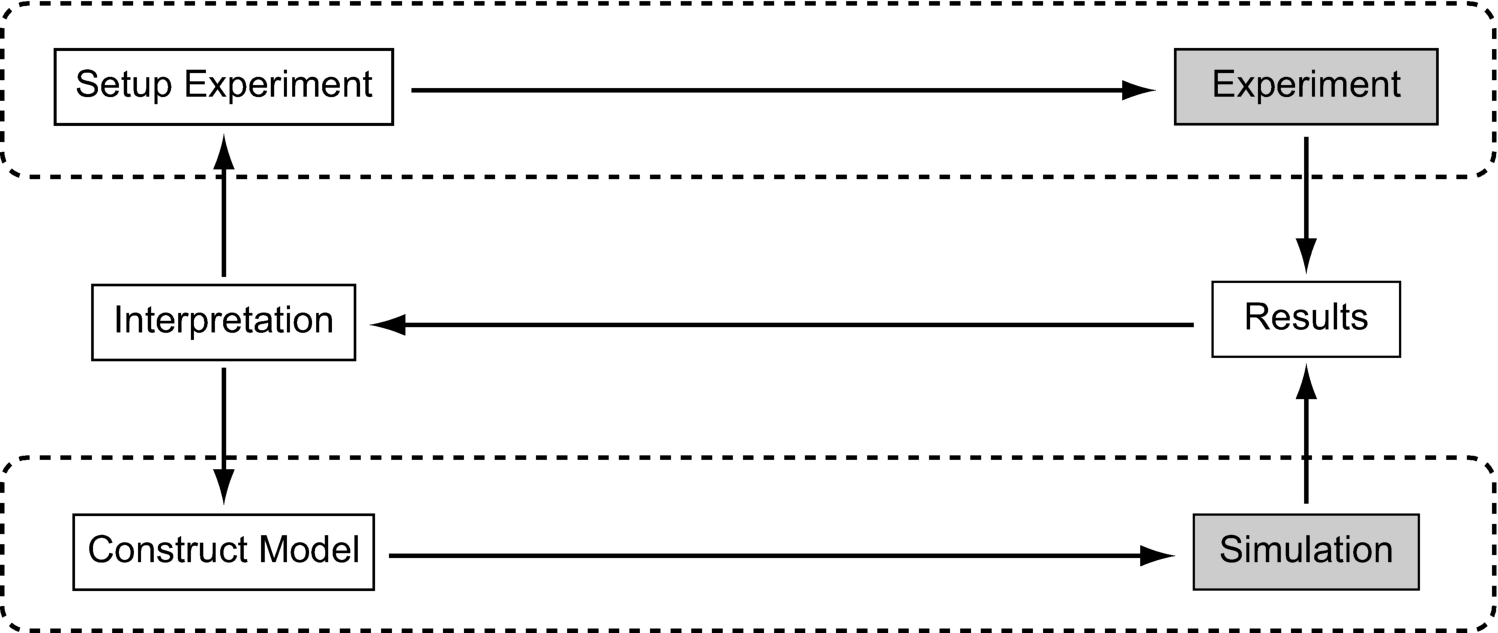
\includegraphics[width=0.45\textwidth]{figures/exp-sim.pdf}
  \end{center}
  \caption{ \small{\textbf{Data flows in science}. Conducting experiments and running simulations are part of two processes delineated by the upper and lower dashed outlines. They are connected by an interposed feedback loop that uses iterative interpretation of results to design new experimental setups and model constructs.}}
    \label{fig:exp-sim}
\end{figure}

From this perspective, simulation provides a framework to organize the understanding of biological systems. The software architecture introduced here (described in following subsections) is designed to support the lower loop within Figure~\ref{fig:exp-sim}. It was developed to resolve the complexities associated with continual addition of functionality to a simulator. To reiterate, historically, simulators have become monolithic and it has become increasingly difficult for users and developers to maintain and extend them. The logical consequence is that user workflows are often similarly degraded. A further problem is that contemporary simulator scripts are typically unstructured in the sense that a biological model is mixed with other code that defines and controls inputs, outputs and simulation configuration~\citep{cannon07:_inter}.

In response to these circumstances, in an effort to avoid the bureaucratic overthink of ``mega-projects" by bypassing the epistemological and methodological metaphors often associated with the workflows of such juggernaut brain research~\citep{fan19}, a five step “ideal user workflow”, or user workflow has recently been proposed~\citep{cornelis12}. 

\begin{figure}[h!t]
  \begin{center}
    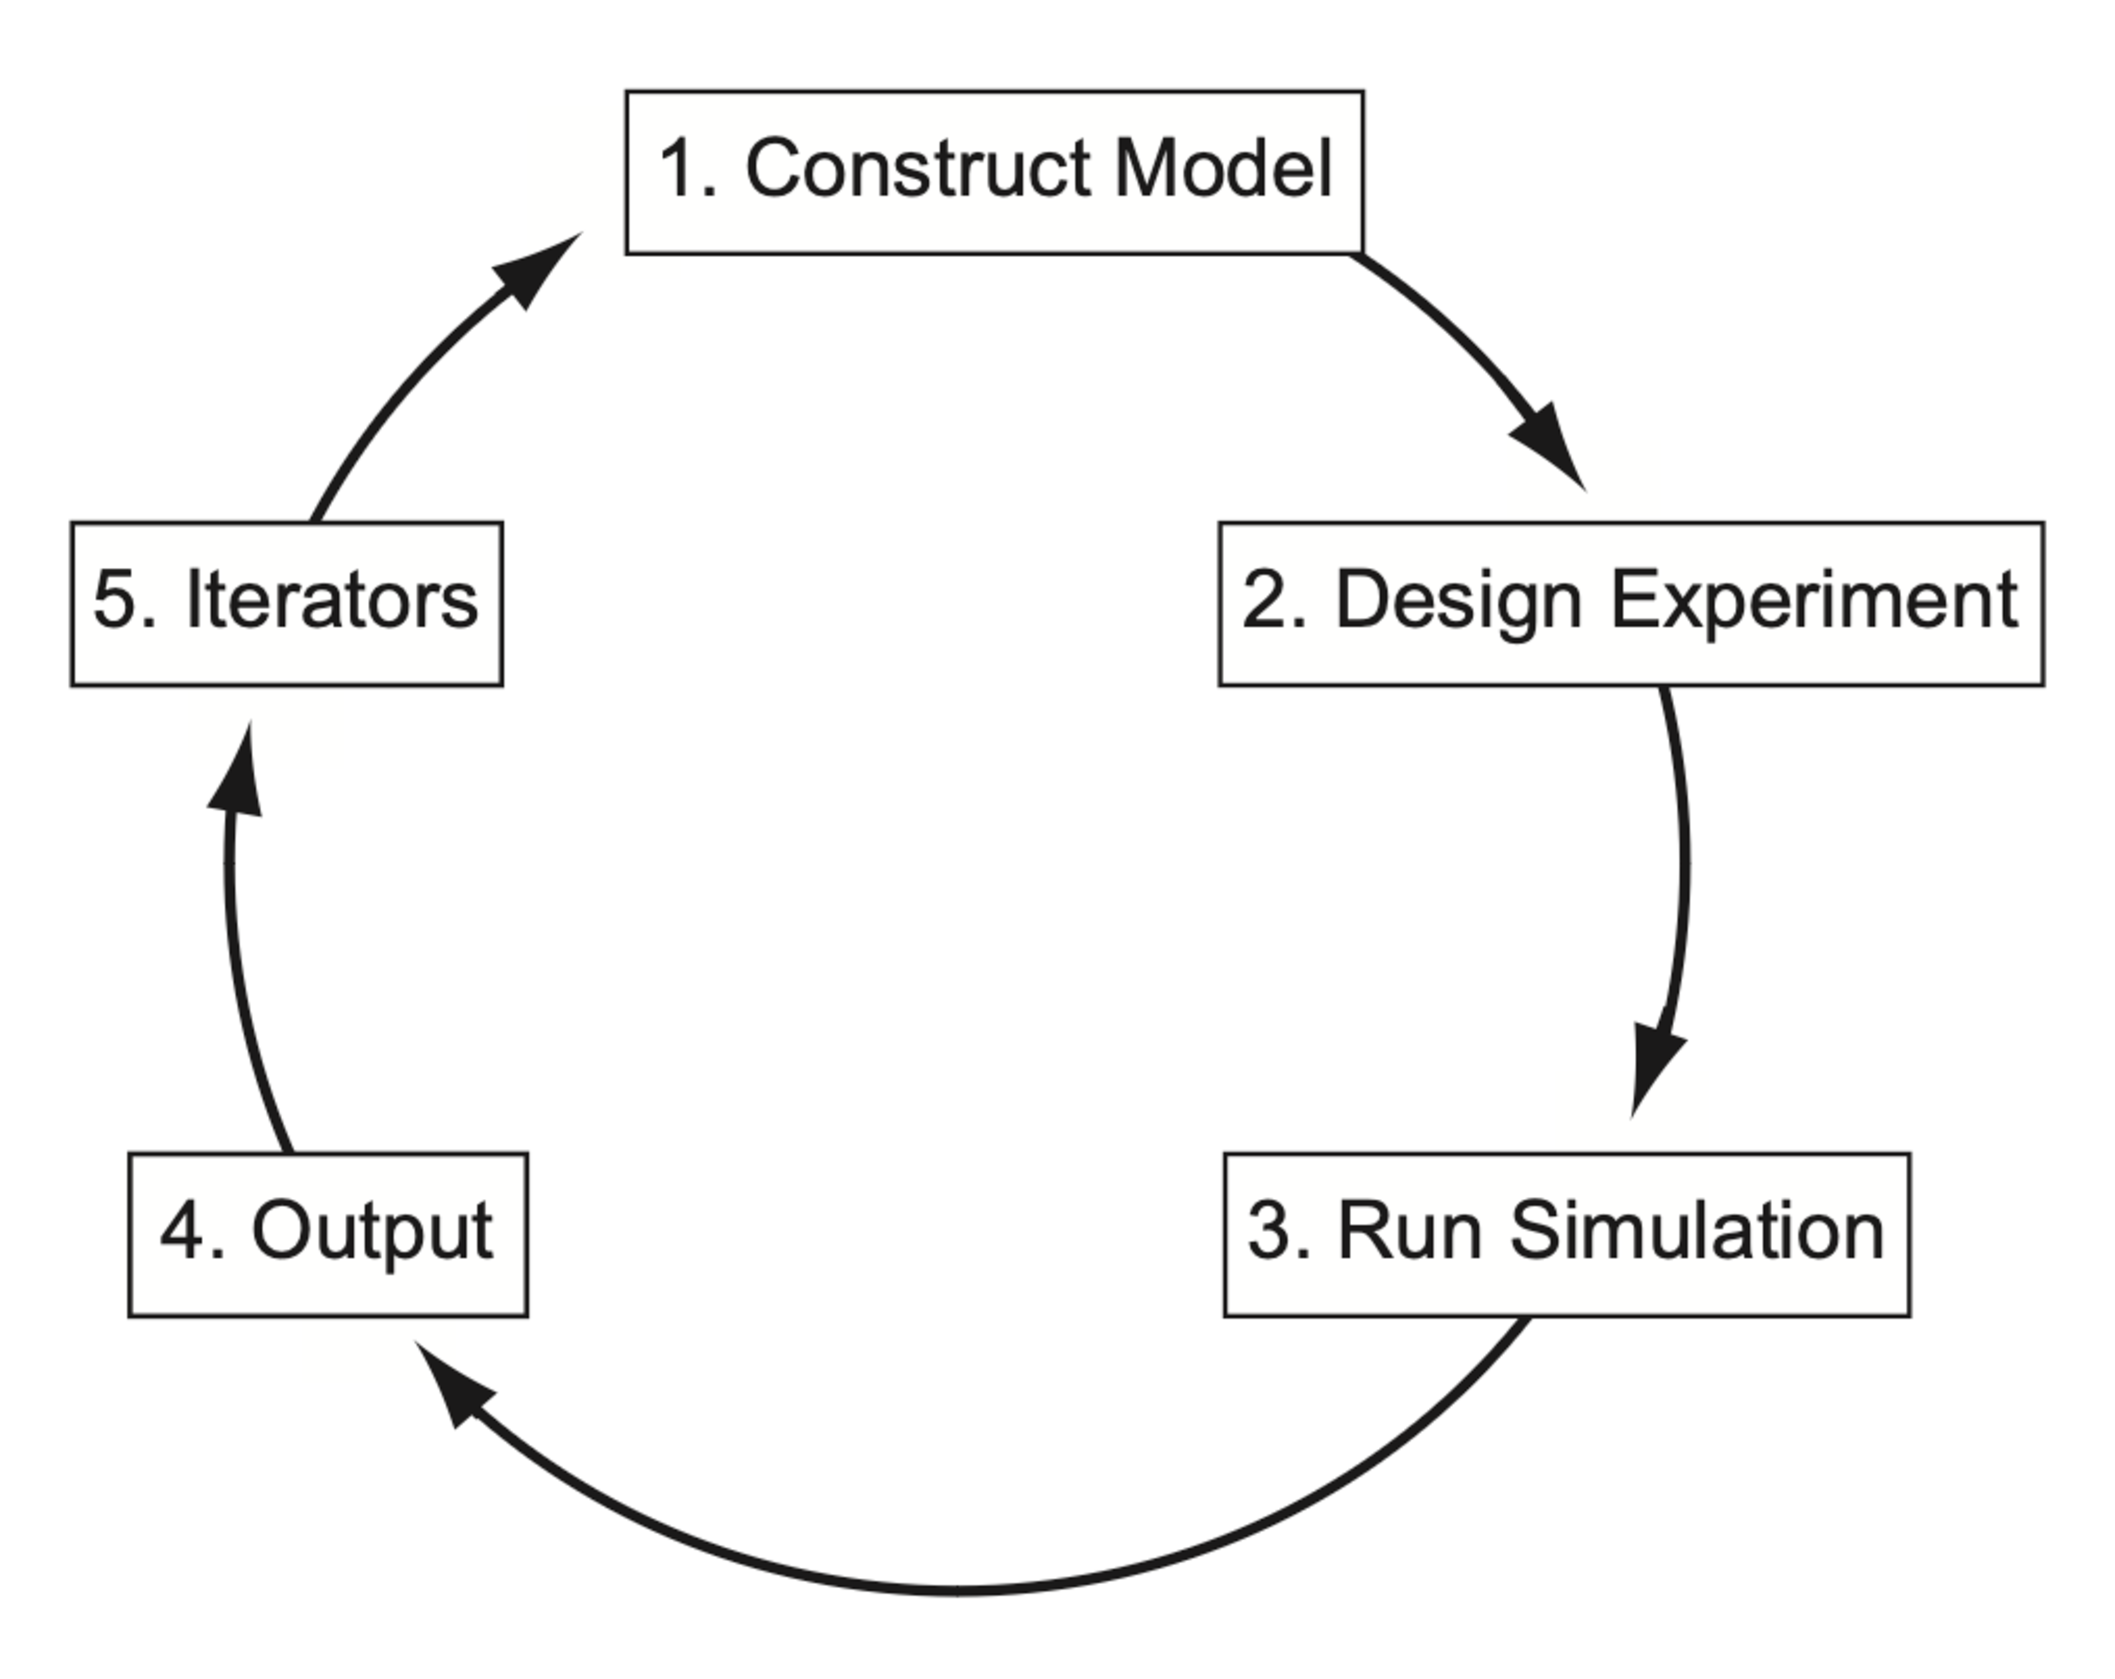
\includegraphics[width=0.45\textwidth]{figures/user-workflow.pdf}
  \end{center}
  \vspace*{-\lineskip}
  \caption{ \small{{\bf The five steps of the ideal user workflow.} {\textbf{1.\,Construct Model:} Simple models can be created directly within the GENESIS$^*$\,\textit{G-Shell} by entering commands. More complex models can be imported into the\,\textit{G-Shell} from either the GENESIS model libraries or from external model libraries. The model can also be explored, checked, and saved. Changes made to the components of a model during a research project include changes to connectivity, cell morphology (e.g. spines), and membrane conductances. \textbf{2.\,Design Experiment:} Set model parameter values specific to a given simulation, the stimulus parameters for a given simulation run or 'experiment', and/or the variables to be stored for subsequent analysis.} \textbf{3.\,Run Simulation:} Configure runtime options, check, run, reset simulation, and save model state. The model state can be saved at any simulation time step to allow it to be imported into a subsequent GENESIS session. Output is flushed to raw result storage for subsequent data analysis. \textbf{4.\,Output:} Check simulation output and the validity of results to determine whether simulation output exists in the correct locations. Output can be analyzed either within GENESIS or piped to external applications such as Matlab, Grace, or Mathematica. \textbf{5.\,Iterators:} Close the loop between output of results and model construction in the GENESIS users workflow. Iterators connect experimental results and model output and include for example, automated construction of simulations and batch files, static parameter searching, and active parameter searching using the dynamic clamp. $^*$\,Version 3.0.}}
  \label{fig:user-workflow}
\end{figure}
%\FloatBarrier

This workflow (see Figure~\ref{fig:user-workflow}) organizes the sequence of activities typically employed for the development and simulation of a computational model, including data generation and analysis.  It consists of five steps: 1.\,Construct model, 2.\,Design experiment, 3.\,Run simulation, 4.\,Analyze output and 5.\,Iterate.  Such a workflow allows the model under investigation, the tools used to perform the investigation and the operations performed during a simulation to be distinguished. These categories correspond to the approaches to computational modelling previously identified by Marr.  

%% For clarification, in the biological domain we refer to ‘multi-level’ (level), in the modelling domain we refer to ‘multiscale’ (scale), and in the software domain we refer to ‘multi-layer’ (layer).
%%\FloatBarrier %% will force figure to specified location
Here, the workflow paradigm is extended by introduction of an organizing principle, the “cognitive workflow”. This workflow describes the process whereby a cognitive abstraction is transformed into an implementation by the conversion of a mental model into a physically instantiated simulation. In doing so, the characteristic labels that historically have come to be associated with descriptions of the classical approach to neurobiological computational simulation have been modified. This important evolutionary step aims to avoid the imposition of interpretations onto the putative structure, contents and functions of neural tissue. In other words, the aim is to minimize the teleology of an explanatory computational model devolving into a merely descriptive demonstration model.

To this end, each step in a given cognitive workflow can be expanded into a matrix where columns span the range of structural detail available at a given resolution of simulation.  As one example of such a workflow, here \ldots  The other steps in the cognitive workflow can similarly be expanded to collectively give a comprehensive framework for scale-independent modelling.

If it is accepted that: (1) a scale-independent approximation can be abstracted at each resolution of a system and disjointly partitioned from its environment~\citep{Bertalanffy:1973zr, Heylighen:2006vn}, and (2) the biological domains implied by Figure~\ref{fig:multi-scale-taxonomy} are plausible, then it is apparent that even a realistic neuron model comprised of at least a soma and dendrites, that includes channels and synapses, is a model simulated at multiple resolutions.

Original location of Figure~\ref{fig:multi-scale-taxonomy}

Thus, one example of a cognitive workflow that facilitates such a path from the cognitive to the physical is given by the top row in Figure~\ref{fig:mental-model-simulation-path} (Biology \textrightarrow\,\,Computer Science).  In this figure, the column to the left gives domains of interest (where the domain identifies the object or event under investigation) and lists domains of biological organization, the column to the right lists the equivalent domains of the software and hardware (operations performed during the investigation), and the central columns give the nature of the mathematical implementation or algorithm (tools used to perform the investigation).  The column items in each row give examples of possible simulator functionality at the given resolution.

\begin{figure}[h!t]
  \begin{center}
    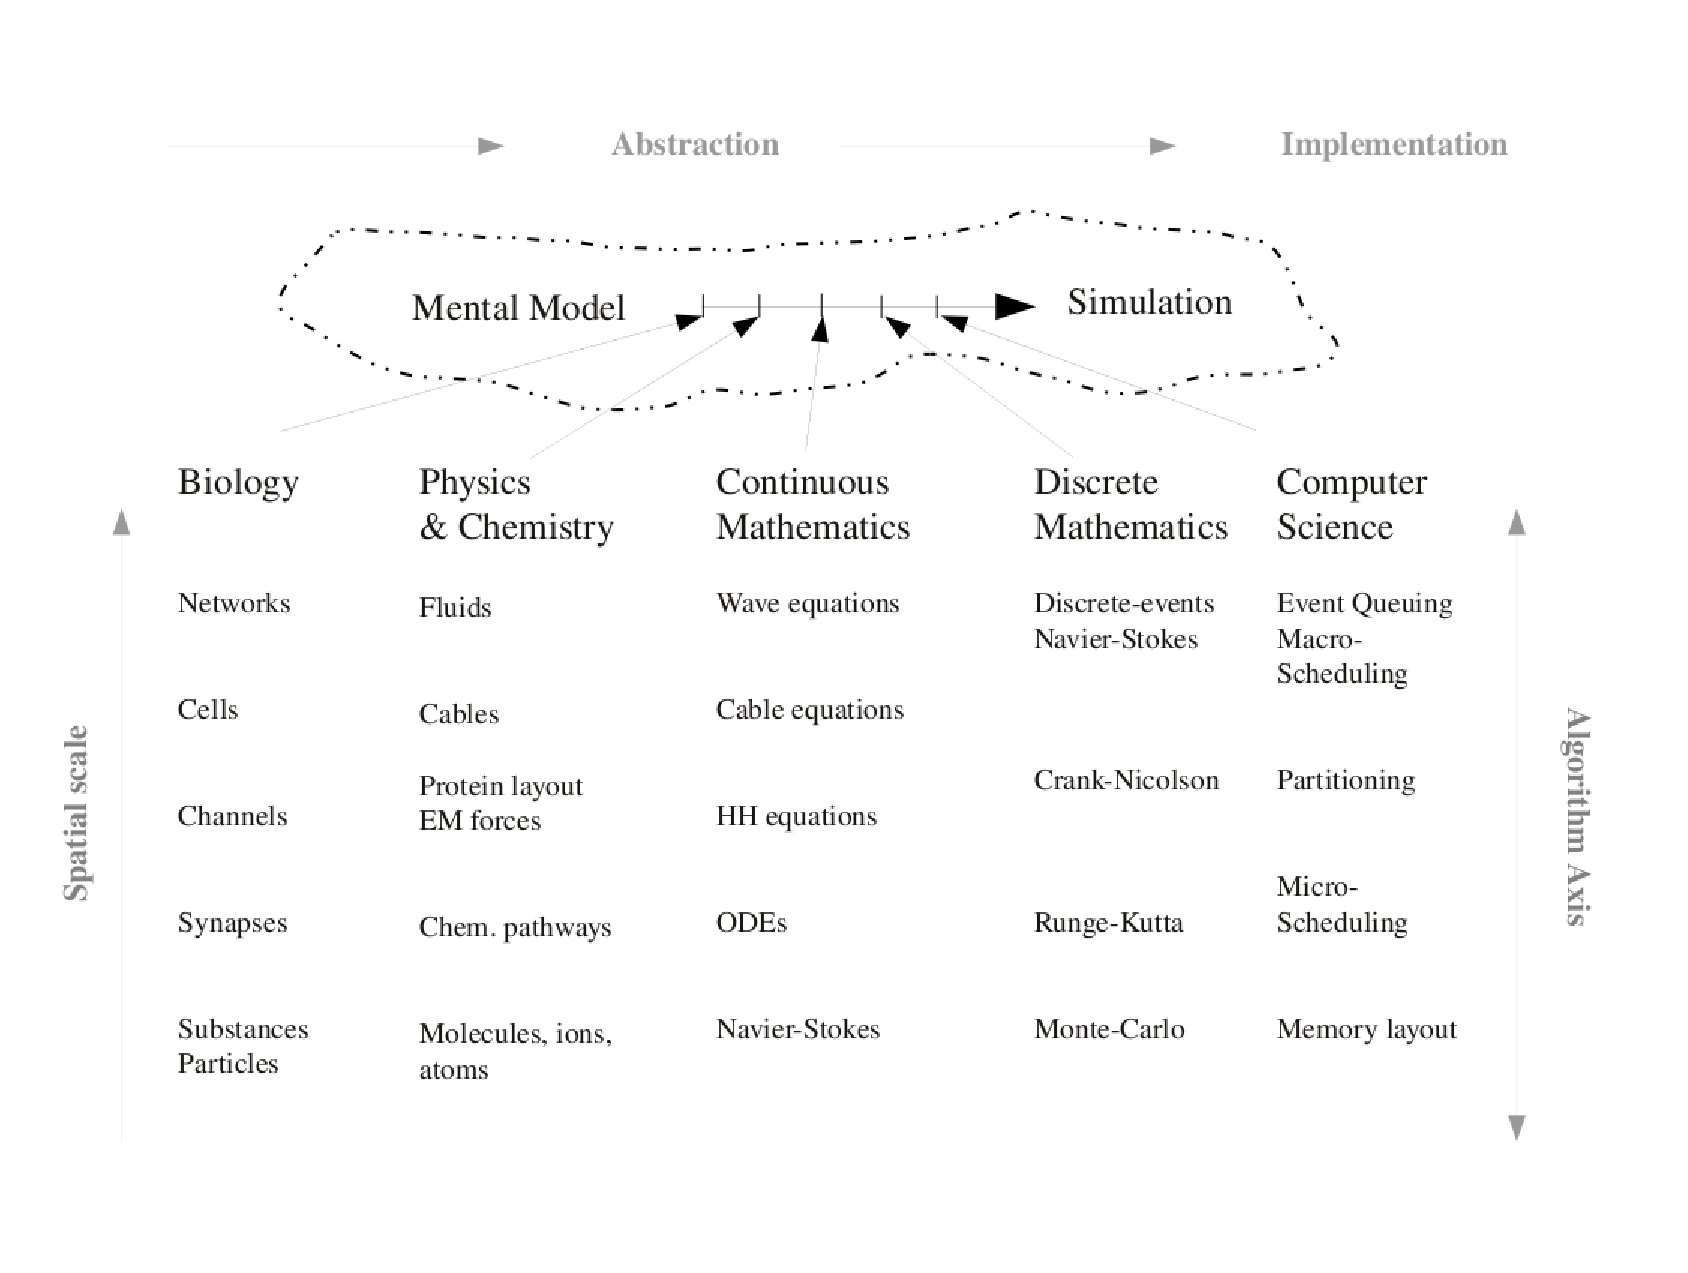
\includegraphics[width=0.45\textwidth]{figures/NS-abstraction-implementation.eps}
  \end{center}
  \caption{ \small{\bf Examples of different cognitive paths from mental model to simulation for different spatial scales.}  Each horizontal path first abstracts the model to a mathematical representation.  This is then followed by how this mathematical representation is implemented in computer software.  The different spatial scales at the left result in the requirement for different algorithms when implementing the computer software.  Each graphical representation of a research topic in the model taxonomy results in researchers applying several cognitive paths that are specific to their methodological workflows (as opposed to their mathematical solutions).  As a consequence the integration of (the results of) different research topics in the model taxonomy requires to trace back on the these cognitive paths.  }
  \label{fig:mental-model-simulation-path}
\end{figure}

The multidimensional framework implied by Figures~\ref{fig:multi-scale-taxonomy} and~\ref{fig:mental-model-simulation-path} is based on the relationships between the schemas outlined by Marr, C\&S, and the user and cognitive workflows described here. These relationships are used to develop a novel and simplifying approach to the simulation of scale-independent models.

Based on the foregoing descriptions and discussions of the multi-dimensional complexity associated with modelling biological structures and functions as ‘simple’ as a single neuron, the features of the reconfigured GENESIS simulator (G-3 -- http://genesis-sim.org) relevant for scale-independent simulation are described.  Together with several scripting examples, it is shown how primary components of G-3 transparently support scale-independent simulation within the various biological resolutions of cells, channels, and synapses (see Fig.~\ref{fig:mental-model-simulation-path}). In short, G-3 provides a scale-independent framework for computational neuroscience that resolves the problems associated with multiscale simulation.

\subsection{Structural Overview of the CBI Architecture}
\label{subsection:CBI-architecture}

The Computational Biology Initiative Federated Software Architecture (CBI architecture) is defined as a modular paradigm that places stand-alone software components into a set of logical relationships \cite{cornelis12}.

In doing so, it defines a modular framework that provides the
necessary parts of a simulator. The architecture takes its name from the Computational Biology Initiative at the University of Texas at San Antonio, where development was first initiated.

\begin{figure}[ht]
\begin{center}
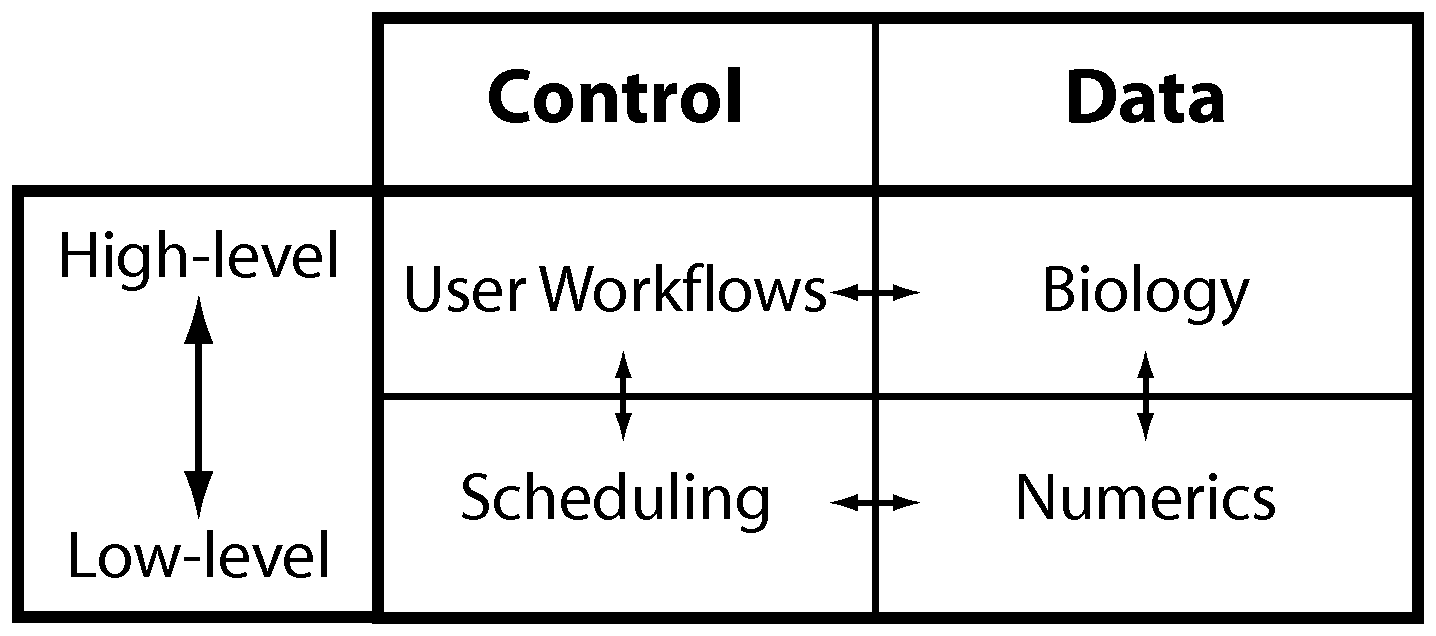
\includegraphics[width=0.45\textwidth]{figures/pone.0028956.g002.png}
\end{center}
\caption{\small{\textbf{Principle concerns.} The four fundamental building blocks of a simulator are distinguished by separating (i) Data from control, and (ii) High level biological concepts from their mathematical implementation. In a federated architecture the only allowed interactions between modules are those indicated by the vertical and horizontal arrows. Diagonal interactions are forbidden as they ultimately lead to interactions that result in the evolution of a monolithic software architecture.}}
\label{fig:concerns}
\end{figure}

A schema identified by separation of concerns (Fig.~\ref{fig:concerns}, see \cite{cornelis12} for details) is expanded in Figure~\ref{fig:cbi-architecture-simple} to give the modules that form the building blocks of the CBI architecture.  The schema retains the four quadrants of simulator functionality identified by the separation of concerns, including separation between control and data  and the notions of high-level representations for biology and low-level data for numerics (Fig.~\ref{fig:cbi-architecture-simple}: indicated by vertical and horizontal dashed lines, respectively).

Notably, the integrity of the simulator is maintained by only allowing interactions between vertically and horizontally located modules. Diagonal interactions are forbidden as they foster the mixing of functionality across different resolutions and typically lead to monolithic software applications. Ultimately, it is this partitioning of simulator functionality that lies at the core of simulator extensibility and provides the architectural foundation for transparent scale-independent simulation.

\begin{figure}[ht]
\begin{center}
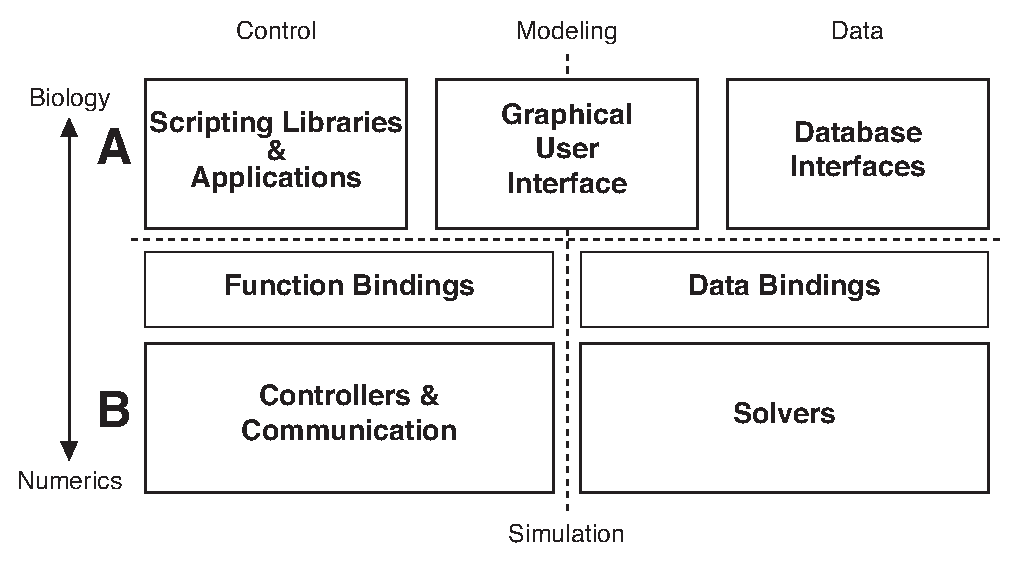
\includegraphics[width=0.45\textwidth]{figures/cbi-architecture-simple.eps}
\end{center}
\caption{ \small{\bf Overview of a federated software architecture:}
  The primary functional modules defined for the CBI federated software architecture are illustrated.  Control modules are given to the left and data modules to the right.  A. The top layer contains conceptual data and controls representations of the biology of a model. B. The bottom layer contains representations that are
  numeric and thus close to the hardware.  The middle or intermediate layer bridges between these `biological' and `numerical' layers in a CBI compliant simulator. Importantly, Control (Scripting Libraries \& Applications) and Data (Database Interfaces) modules can interact either directly or via the Graphical User Interface. }
\label{fig:cbi-architecture-simple}
\end{figure}

The CBI architecture is referred to as being `federated' as it extends
the modular approach associated with the development of single
applications to the functional integration of otherwise independent
applications.  Federation aims to provide a unified interface to
diverse applications and ideally make them look like a single
system to the user. In doing so, it provides transparency, heterogeneity, a high
degree of function, autonomy for the underlying federated sources,
extensibility, openness and the possibility of highly optimized
performance (see \cite{federated-2002-xyz}). Here, extensibility is defined as a system design
principle where an implementation takes into consideration future
developments. An extensible system is one that includes mechanisms for
expanding or enhancing the system with new capabilities without having
to make major changes to system infrastructure. 

Enhanced application interoperability and performance is available
through the use of flexible high-level scripting languages that support
diverse workflows, low-level application programmer interfaces
(API)s and application binary interfaces (ABI)s (see \cite{Cornelis:2011fk}).

% For completeness, we note that northbound and southbound interfaces
% are indicated in this figure. Northbound interfaces conceptualize
% lower level details, whereas, the southbound interfaces decompose
% the concepts in technical details, which are mostly specific to a
% single component of a software architecture. Northbound interfaces
% normally communicate with southbound interfaces of higher level
% components and vice versa. By convention, north- and southbound
% interfaces are drawn at the top and bottom of an architectural
% overview, respectively.

In summary, the CBI architecture provides a template for software
development that, at its core, contains a simulator.  Additionally,
the modularity and layering of the architecture simplifies connection
to independent applications related to model construction
and instantiation and the analysis and display of simulation output.

\subsubsection{Behavioural View of the CBI Architecture}

Figure \ref{fig:cbi-architecture-expanded} expands Figure \ref{fig:cbi-architecture-simple} to give more
detail of the structural relationships between the different modules and
sub-modules of the CBI architecture (previously described in \cite{cornelis12}). The behavior of
the CBI architecture is defined by the functional and dynamic
connectivity provided by these individual modules. This behavior is now introduced within the context of the user workflow.

\begin{figure}[h!t]
  \begin{center}
    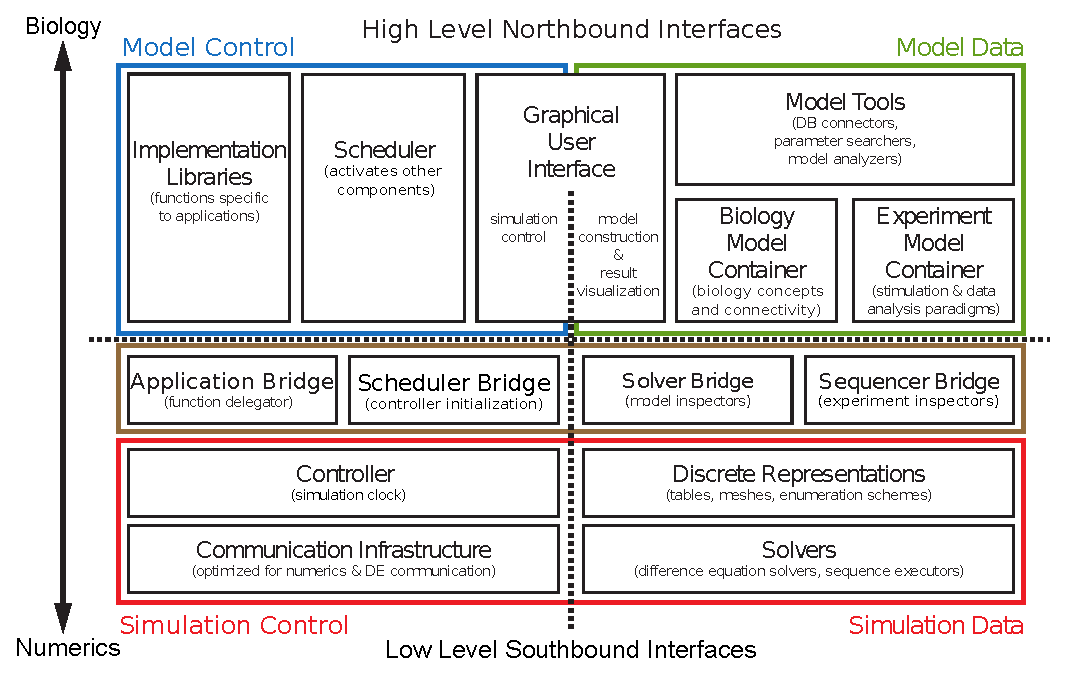
\includegraphics[width=0.45\textwidth]{figures/cbi-architecture-expanded.eps}
  \end{center}
  \caption{ \small{{\bf Detailed view of the Computational Biology Initiative
      federated software architecture.} Relationships of sub-modules
    within each of the primary functional modules given in Figure
    \ref{fig:cbi-architecture-simple} are illustrated.  North bound interfaces group
    and conceptualize the details of the modules and interact with
    south bound interfaces of higher level modules.  Steps 1--3 of the
    user workflow induce data cycling between the
    upper layers (blue and green boxes) and lower layers (red box), see Figure~\ref{fig:user-workflow} for details.
    Ultimately, the two layers interact to implement a single simulation.
    By design, any type of model including multiscale models will
    exhibit this data cycle. In contrast to previous versions of GENESIS and
    other neuronal simulation platforms, the design of G-3 is
    fundamentally modular, separating different functional components
    of the simulator into their own modules. Importantly, G-3
    separates model descriptions from their mathematical representations.  This simplifies the
    implementation of new {\bf Solvers} and other run-time software
    components. The communication infrastructure connects different
    {\bf Solvers} to simulate different parts of a model and can `upscale' or `downscale'
    numerical data as needed. Additional detail is given in \cite{cornelis12}.}}
  \label{fig:cbi-architecture-expanded}
\end{figure}

%\subsubsection{Data-flows in the CBI Architecture}

%A (G)UI translates user actions into a family of events that propagate
%to other components of a software architecture, impact the internal
%states of these components, and direct the data flows between them.
%In the CBI architecture each software component is specialised in
%implementing one particular function and performs the defined
%operations on the data it is passed.
%A functional architecture is an overview of a software system that
%identifies the global functions of the system.  These functions define
%the scope for experts for improvement of the system as a whole.  The
%CBI architecture is structured according to low-level vs. high-level
%functions in the system complemented by the data and control
%functions.  As a consequence, a feature of the CBI architecture is
%that rich data flows occur between software components, but not
%necessarily within them.
During the phase of model construction prior to simulation, users combine models from files and databases.  When the simulation runs, the numerical {\bf Solvers} perform the calculations of a simulation, and save the output back to files and databases.  When these two steps are combined they imply a cyclic data flow from files and databases to the {\bf Solvers}.
%  Here we explain how user actions and data flows relate to one another in the CBI architecture and define the overall behavior of an implemented software system.

In more detail, as a result of Steps 1--3 of the user workflow (construct model, design experiment, run simulation, see Fig.~\ref{fig:user-workflow}), data flows both through and between software components. The cycle described here is for a single neuron simulation, however, all scales of model will exhibit similar activity.

Once Step 3 is completed, data generated by dynamic states of the model are available through databases and files. Consequently, there is no requirement to query software components that deal with numerical data. This provides an operational barrier to assist with preventing incremental conversion of a CBI compliant simulator to its monolithic equivalent.

In Step 4 of the user workflow (output), while maintaining the integrity of the separation of concerns, the availability of any model data from the {\bf Biology\,Model\,Container} and the functionality of {\bf Scripting\,Libraries\,\&\,Applications} can be used to connect the CBI architecture to external tools, for example Matlab (to implement output analysis).

At Step 5 of the user workflow (iterate), simulation output data and model parameters and structure available in the model containers can be combined, for example, to provide automated script generators for the creation of batch simulations. Importantly, at this stage of the workflow, the back-ends of the CBI architecture (indicated below the dotted horizontal line in Figures \ref{fig:cbi-architecture-simple} and \ref{fig:cbi-architecture-expanded}) are unavailable. 

%Intermediate results may be analyzed or aggregated by
%analysis libraries, e.g. for signal analysis and binning of spikes.
%These libraries are accessible to the CBI architecture from the {\tt
%  Scripting Libraries \& Applications} software component.

%\paragraph{Running a Single Cell Model:}

%When a user wants to learn more about the electrophysiology of an
%existing cell model, it must be instantiated, the stimulation and
%output protocols configured, the simulation run, and the results
%interpreted.

%In Step 1 of the user workflow, the GUI is opened and a cell
%model is selected from a database listing of available models.
%Internally, model selection is translated into an event that instructs
%the {\tt Biology Model Container} to load a selected model from a
%database and store it in memory using data structures for efficient
%storage and retrieval by other modules.  During initial inquiry, a
%user may typically be interested in derived model parameters such as
%the total surface area of a neuron, with and without spine correction,
%while a sophisticated GUI can also present a table of the channels
%employed in the model along with their conductance densities and
%reversal potentials.  More dedicated queries related to specific brain
%areas or neuron types are supported by the {\tt
%  Scripting Libraries \& Applications} module.

%%A model can be queried in this way when it is stored by
%%the {\tt Biology Model Container}.

%A typical example of Step 2 of the ideal user workflow is the design
%of an experiment that applies current injection pulses to a neuron's
%soma and defines simulation output as the somatic membrane potential
%and somatic transmembrane currents.  The {\tt
%  Experiment Model Container} stores the definition of the current
%pulse amplitude and duration, which is translated by a {\tt
%  Sequencer Bridge} to a sequence of simulation-time events prior to
%the start of a stimulation.  These events are then executed by the
%{\tt Command Sequence Executor} during a simulation.

%Running the simulation in Step 3 of the ideal user workflow starts
%with the {\tt Biology Model Container} examining a stored model to
%determine model time constants or other parameters that are relevant
%for the accuracy of a numerical simulation.  The {\tt Solvers} then
%fill their data structures with parameter values optimized for
%simulation, for instance a Crank-Nicolson solver can multiply the
%membrane capacitance with the time step during this initialization
%phase instead of at every simulation time
%step \cite{borg-graham00:_addit_effic_comput_branc_nerve_equat}.  For
%this, the memory image of a model must first be expanded into a
%representation that includes the mathematical equations and parameters
%relevant to the given simulation but, for instance, does not include
%the spatial layout of segments as this is not required by the {\tt
%  Solvers}.  (Note: `Segment' is a high level term employed to describe different parts of the biological model of a dendritic morphology. The equivalent low level (computational) term is `compartment'. It refers to the numerical representation of a segment.) This behavior is different from that of existing
%simulators, e.g. GENESIS 2. Such simulators do not make an explicit
%distinction between internal data structures for model representation
%and data structures for computation.  Consequently, they often
%generate redundant data during the initialization of a simulation.

%In network simulations the {\tt Solvers} employ the {\tt
%  Connectivity Translator} to initialize its simulation-time
%communication data structures and to connect to the {\tt
%  Communication Infrastructure}.

%When a user instructs the simulator to start a simulation, for
%instance by pushing a button in a GUI, the {\tt Controller} generates
%a list of instantiated {\tt Solvers}.  It then advances the simulation
%clock and requests each {\tt Solver} to update its internal state.
%The {\tt Communication Infrastructure} connects the {\tt Solvers} for
%efficient communication of the solved variables.  {\tt Solvers} that
%were configured for output, save results to a file.  When the
%simulation finishes, either by user action or following a preset
%simulation period, output buffers are flushed to disk.

%The independence of the {\tt Solvers} in the CBI architecture not only
%allows for better optimized implementations, but also enables
%additional simulator functionality such as serialization of the model
%state to a file.  This allows a simulation to be resumed at a later
%time and reduces the total simulation time of a complex model if it requires
%a calibration phase prior to the application of an experimental
%protocol.

%%During Step 4 the dynamic state of the model is available from the files and databases for further analysis.

%% Steps 4 and 5 are complementary to Steps 1-3 of the ideal user workflow.

%%The data cycle between databases and files, and the solvers in Steps
%%1-3 of the ideal user workflow results in all simulation simulation output
%%is available through these databases and files.  Once these steps
%%have been completed, the back-ends of the CBI architecture are not
%%available anymore.  The simulation result data can then be combined
%%with the model parameters and structure available in the {\tt
%%  Biology Model Container} through {\tt
%%  Scripting Libraries \& Applications} to implement Step 4 and 5 of
%%our ideal user workflow.

%As a result of Steps 1--3 of the ideal user workflow, data flows both
%through and between software components that conform to a CBI
%architecture: the data cycles between databases and files, and
%back-end {\tt Solver}s.  Here we have described this cycle for a single
%neuron model and, as we briefly noted, it also occurs for network
%models.  By design any type of model including multiscale models
%will exhibit this data cycle.

%In Steps 4 and 5, the availability of any model data from the {\tt
%  Model Container} and the functionality of {\tt
%  Scripting Libraries \& Applications} can connect the CBI
%architecture with external tools while maintaining the integrity of
%the separation of concerns.
%%The laterality of the software component connectivity activated during Step 4 is not an issue.
%{\tt Scripting Libraries \& Applications} connect to external tools
%such as Matlab to implement output analysis.
%%  Integration, at Step
%%4 of the ideal user workflow, with software platforms such as RTXI
%%make direct interaction with experiment possible.
%They also allow simulation output data to be combined with the model
%parameters and structure available in the {\tt
%  Biology Model Container} to implement Step 5 of our ideal user
%workflow, for instance to provide automated script generators for the
%generation of batch simulations.  Importantly, at this stage of the
%workflow, the back-ends of the CBI architecture (indicated below the dotted
%horizontal line in Figures~\ref{fig:cbi-architecture-simple}
%and~\ref{fig:cbi-architecture-expanded}) are unavailable.  Once Step 3
%is completed, all the data of the dynamic state of the model are
%available through databases and files.  Consequently, there is no
%requirement to query the software components that deal with
%numerical data. This ultimately prevents the implementation of
%diagonal interactions in the software and the creation of a monolithic
%simulator.

%% are technically unrelated to a simulation run and may
%%fall outside the scope of the CBI architecture.  On the other hand
%%{\tt Scripting Libraries \& Applications} may connect to external
%%tools such as Matlab to implement output analysis and include script
%%generators for automation of batch simulations and platforms such as
%%RTXI for a direct connection with experiments.

%%For convenience one could implement a short-cut diagonal into the CBI
%%architecture for implementation of aspects of Steps 4 and 5, and for that matter other Steps, but this ultimately would limit the functional scope of the resulting simulator.

%%All model data is available through the model container and the output (files or databases).  

%%Modules plugged in during Step 4 have access to all data via the model container.

\subsection{GENESIS 3.0}

The software architecture developed for G-3 supports a capacity for federated and modular software development that directly enables multiscale modelling.  Furthermore, its structure also supports the direct interaction with, or embedding of, models at different resolutions.  During model construction this is accomplished through the reconfiguration of the internal model storage format, while during simulation run-time it occurs through specific software modules that create intermediary representations of variables present at multiple resolutions (described in more detail below).

Several explicit features of G-3 allow new software components to be rapidly incorporated into the simulator: (1) modularity of the CBI architecture supports the development of new {\bf Solvers} independently of other software components. This encourages full focus on the mathematical aspects of {\bf Solvers} and their implementation and leads to better optimization, (2) the {\it Developer\,Package} facilitates integration of new {\bf Solvers} into the build system of G-3 enabling immediate regression testing, (3) easy extension of the configuration of the internal model storage format to establish new declarative model tokens and parameters recognized by new {\bf Solvers}, (4) easy construction of an interface between the internal data storage format and the core of new {\bf Solvers}, and finally, (5) a communication software component that creates simulation run-time interfaces between {\bf Solvers}.

Solvers currently available in G-3, starting at the highest level, include: {\bf DES}, a discrete event queuing and distribution infrastructure for network modelling, {\bf Heccer}, a single neuron solver, {\bf Chemesis-3}, a simple reaction-diffusion system solver, and {\bf Experiment}, which provides simulation-time components for current injections, time-tables, and output.

%\subsubsection{Extending GENESIS-3}

%The G-3 documentation systems describes the procedures used for G-3
%extension.  Extending G-3 can involve the implementation of a new
%solver, or, when the required functionality is tangential to an
%existing solver, it can require source code additions to an
%pre-existing software component.  Here we describe the integration of
%a new solver, ie. the steps followed for the implementation of
%{\bf Chemesis-3}.

%\begin{enumerate}[noitemsep,nolistsep]
%\item The developer package integrates the different software
%  components of G-3.  The definition of a new component ``chemesis3'' in
%  the developer package allows for its smooth integration with other
%  G-3 software components such as the model-container.
%\item The implementation of the core of a new solver is independent of
%  the development of other software components.  This allows full
%  focus on the mathematic aspects of the solver and their
%  implementation.
%\item Optionally, the model-container can be extended with new tokens
%  that are specific to the new solver.  Configuration of the
%  model-container defines the new tokens and their parameters.
%\item An interface must be written between the model-container and the
%  core of the solver.  The model-container defines an API that makes
%  abstraction of the biological structure the model.
%\end{enumerate}

\subsubsection{The Model Containers}

\paragraph{Biology\,Model\,Container:} Provides a solver-independent internal storage format for models. Stores biological entities and end-user concepts and annotates the structures and concepts of a model with biological, physical, and mathematical quantities. By ``containing" the biological model, the {\bf Biology\,Model\,Container} relieves the implementation of the numerical core of a solver from the pressure of user-friendly model representation.

Because all model components are interactive parts of a single model-container \cite{cornelis12}, existing and new G-3 {\bf Solvers} can be incorporated to simulate different aspects of the same model.  This {\em scale-linking} functionality of G-3 instantiates dedicated run-time software components that contain intermediary representations of solved variables able to pass both {\em higher resolution} and {\em lower resolution} values to {\bf Solvers} operating at different resolutions.
%  Technically, in the case of {\bf Chemesis-3} and the
%linear cable solver, for example, these modules calculate weighted
%space-time averages.
It is through this computational mechanism that the {\bf Biology\,Model\,Container} supports transparent construction and simulation of multiscale models.

\paragraph{Experiment\,Model\,Container:} Stores a model of a stimulus paradigm and desired output parameters. It also defines and stores a hierarchical sequence of stimulus-related
actions (e.g. start and stop time of a current injection) and their dependencies.

Finally, it is noted that the model containers define models in a purely declarative,
extensible language.

\subsubsection{The Neurospaces Description Format}

The Neurospaces Description Format (NDF) file format developed for the model containers was originally designed as a file-based user-editable declarative interface to the {\it hsolve} method used by GENESIS-2 \cite{cornelis03:_inter_model_space_simul_space,beeman12:_years_comput_neuros}. Subsequently, its single neuron modelling functionality was expanded with network modelling capabilities.

The NDF file format is indicated by the {\tt .ndf} file name extension. This format integrates and extends the previous GENESIS {\tt .p} and {\tt .g} declarative file formats. NDF files are purely declarative and can be stored in a model database. In an NDF file, a
model exists as a hierarchy of tokens, each representing a biological component.  Each component is associated with a set of physical processes and can have parameters and shared variables (described in more detail below).  This feature allows the NDF format to support
both multi-level and multiscale modeling.
% To introduce the format we now outline the general structure of an NDF file.

G-3 supports the construction of NDF files. These files define the different components of a model.  They simplify and expedite model development by being shared between and imported into other NDF files, or used to create NDF libraries. NDF libraries can be linked and used to store model lineages, thereby curating and representing different levels of neuronal morphology and/or electrophysiological function.
%Models declared in an
%NDF file can be `private' to that file, or `public' and
%available to other NDF files. This mechanism prevents the use
%of certain (private) components, while allowing reuse of other
%(public) components.
These relationships support and control the modular construction of multiscale
models as any given NDF file can depend on other NDF files.

\paragraph{Overview of an NDF File:}
\label{sec:overview-ndf-file}
%We now introduce the basic parts of a simple NDF file that defines a single compartment neuron containing classical Hodgkin-Huxley descriptions of $Na$ and $K$ channels.
An NDF file contains four sections. They are not necessarily filled, but must be present in the given order.  Files have the following general form (described in more detail below).

\begin{center}
 % \begin{boxedminipage}{13cm}
 \begin{tiny}
\begin{verbatim}
    #!/usr/local/bin/neurospacesparse
    //-*- NEUROSPACES -*-
    // default location for file comments
    NEUROSPACES NDF
    IMPORT
        FILE <namespace> "<directorypath>/<filename.ndf>"
         . . . <other files may be imported as required>
    END IMPORT
    PRIVATE_MODELS
    
        ALIAS <namespace>::/<source label> <target label> END ALIAS
            . . . <other aliases may be defined as required>
    END PRIVATE_MODELS
    PUBLIC_MODELS
        CELL <morphology name>
            SEGMENT_GROUP segments
                . . . <morphological details>
            END SEGMENT_GROUP
        END CELL
    END PUBLIC_MODELS
\end{verbatim}
\end{tiny}
%  \end{boxedminipage}
\end{center}

The header section
typically starts with a UNIX {\it interpreter} sequence. It
gives the system specific absolute path to the {\bf Model\,Container} stand-alone executable.
%\begin{verbatim}
%    #!/usr/local/bin/neurospacesparse
%\end{verbatim}
This is followed by optional comments.  The text {\tt NEUROSPACES NDF} marks the start of model definitions.
%The first (optional) declaration flags an appropriate major
%mode and keyword highlighting for Emacs and XEmacs (the Neurospaces Emacs major mode is bundled with the
%  NMC package). The second declaration identifies the file type (here NDF).

The {\tt Import} section
 uses the {\tt FILE} keyword to declare
dependencies on other NDF files.

%, e.g.
%\begin{verbatim}
%    IMPORT
%        FILE <namespace> "<path>/<fname>.ndf"
%    END IMPORT
%\end{verbatim}

The {\tt Private Models} section defines models that are private to a single NDF file.  They may depend on imported public models of other files.

The {\tt Public Models} section defines models that are visible to the NDF files into
which they are imported.
%  Typically, for example, a neuron morphology
%would be located here.
  Public models may depend on private models or
be hard coded.

\paragraph{Physical Processes and Model Parameters in NDF:} Mathematical models can be used to describe physical processes underlying the functional activity of biological entities by associating the physical processes with parameters (fixed during a simulation) and
variables (computed during a simulation).

%A variety of techniques exist to model diffusion and concentrations of
%ions in a (segment of a) dendritic tree.  The simplest case is that of
%the concentration of an ion.
As an example, consider a calcium pool $\mathrm{Ca}^{2+}$ whose concentration
follows an exponential decay according to the equation:

\begin{equation}
  \label{eq:decay-concentration}
  \frac{\mathrm{d}[\mathrm{Ca}^{2+}]}{\mathrm{d}t} = B \cdot I_{\mathrm{Ca}^{2+}}
  - \frac{[\mathrm{Ca}^{2+}]}{\tau}
\end{equation}
where $I_{\mathrm{Ca}^{2+}}$ is an ionic current flowing into a segment
%(here expressed in amperes).  
and $B$ is a decay constant (sometimes referred to as $\beta$), often
found by fitting experimental data \cite{bower98:_book_genes}.
%  In some cases the above equation is used
%as a model for the concentration in a thin shell near the surface of a
%dendritic segment.  In that case $B$ can roughly be approximated with
%the formula:

%\begin{equation}
%  \label{eq:decay-concentration-B}
%  B = \frac{5.2 \cdot 10^{-6}}{A \cdot d}
%\end{equation}

%with $A$ the surface area of the shell and $d$ the thickness of the
%shell, here both expressed in meters (the outer diameter of the shell
%is the same as the diameter of the segment).

In an NDF file calcium decay  can be represented as follows:
%note: based on granule_ca.ndf

\begin{tiny}
\begin{verbatim}
  POOL Ca_concen
    PARAMETERS
      PARAMETER ( concen_init = 75.5e-6 ),
      PARAMETER ( TAU = 0.01 ),
      PARAMETER ( VAL = 2.0 ),
      PARAMETER ( BETA = FIXED
                  (PARAMETER ( value = 1.98e+11 ),
                   PARAMETER ( scale = 1.0)  ))
    END PARAMETERS
  END POOL
\end{verbatim}
\end{tiny}
%As an example, a synaptic current is commonly modelled using a
%second-order differential equation (where in computational neuroscience the right-hand side of the equation
%corresponds to the level of synaptic activation delivered by spikes
%arriving at times $t_i$):
%\begin{equation}
%  \label{eq:second-order-synchan}
%  G'' + \alpha G' + \beta G = S
%\end{equation}
%where $\alpha = \frac{\tau_1 + \tau_2}{\tau_1 \tau_2}$, $\beta =
%\frac{1}{\tau_1 \tau_2}$, and $S = \delta(t - t_1) + \cdots + \delta(t - t_N)$.
%%
%Assuming the initial values $G(0) = 0$ and $G'(0) = 0$, the solution
%to this equation is a dual-exponential equation:
%\begin{equation}
%  \label{eq:dual-exponential}
%  G(t) = \frac{\tau_1\tau_2}{\tau_1 - \tau_2}
%  \cdot (\mathrm{e}^{\frac{-t}{\tau_1}} - \mathrm{e}^{\frac{-t}{\tau_2}})
%\end{equation}
%%\begin{equation}
%%  \label{eq:simple-spatial-cable}
%%  \frac{a}{2R_a}\frac{\partial^2V}{\partial x^2} = C_m \frac{\partial V}{\partial t} + \frac{V}{R_m}
%%  + I_{\mathrm{HH}} + I_{\mathrm{syn}}
%%\end{equation}
%This equation has two parameters {\tt TAU1} and {\tt TAU2}, sometimes
%called the rise and decay time constants, respectively.  Assigning
%values to these two parameters in an NDF file is done as follows:
%%EQUATION_EXPONENTIAL exp2
%%
%%  ...
%\begin{verbatim}
%  PARAMETERS
%    PARAMETER ( TAU1 = 0.50e-3 ),
%    PARAMETER ( TAU2 = 1.20e-3 )
%  END PARAMETERS
%\end{verbatim}
%%END EQUATION_EXPONENTIAL

In the example above, each parameter has a value that is fixed during the model construction phase.  In the general case a parameter can either be a constant value, point to a parameter of another component, or have the value of a function.  For example:

\begin{tiny}
\begin{verbatim}
PARAMETERS
   PARAMETER ( DIAMETER = 0.3 ),
   PARAMETER ( LENGTH = ..->LENGTH ),
   PARAMETER ( SEED = SERIAL () )
END PARAMETERS
\end{verbatim}
\end{tiny}

where {\tt DIAMETER} has a constant value, {\tt LENGTH} is inherited from the parent component (the `$..$' notation is a reference to the parent component), and {\tt SEED} has a value defined by the function {\tt SERIAL()}.  Importantly, neither the NDF file format nor the model container make a syntactical distinction between the parameters and variables of a physical process.  For example, {\tt LENGTH} is neither defined as a parameter with a fixed value nor as a solved variable.  This logic is employed as a numerical value may be a parameter in one model but a variable in another.
%We note that the NDF file
%format supports both the '$..$', and $^\wedge$ notations to
%reference the parent symbol.  (While non-technical people might
%prefer the $^\wedge$ notation,
%technical people will prefer the '$..$' notation.)

When one biological entity modulates the behavior of another, their physical processes share one or more variables.  For example, in the case of a `pool' containing calcium ions, a transmembrane calcium current may raise the concentration of the pool. In this example, the current ({\tt I}) is a variable common to both the conductance and the pool. Such variables, when shared between multiple physical processes, are declared using the {\tt BINDABLES} keyword.

\begin{tiny}
\begin{verbatim}
  BINDABLES
    INPUT I
  END BINDABLES
\end{verbatim}
\end{tiny}
Assuming a calcium current is present under the label {\tt ../cat}, it can be bound to a pool by using a {\tt BINDINGS} clause:
\begin{tiny}
\begin{verbatim}
  BINDINGS
    INPUT ../cat->I
  END BINDINGS
\end{verbatim}
\end{tiny}

%Putting everything together using the {\tt EQUATION\_EXPONENTIAL}
%token to represent the dual-exponential equation, we get the NDF
%snippet that defines a model's component with name {\it exp2}:
%\begin{verbatim}
%EQUATION_EXPONENTIAL exp2
%  BINDABLES
%    INPUT activation, OUTPUT G
%  END BINDABLES
%  BINDINGS
%    INPUT ../synapse->activation
%  END BINDINGS
%  PARAMETERS
%    PARAMETER ( TAU1 = 0.50e-3 ),
%    PARAMETER ( TAU2 = 1.20e-3 )
%  END PARAMETERS
%END EQUATION_EXPONENTIAL
%\end{verbatim}

%In this example, the order of the clauses of {\tt BINDABLES}, {\tt
%  BINDINGS}, and {\tt PARAMETERS} was chosen for readibility.  

\paragraph{multiscale Models in NDF:} The NDF file format is loosely based on GENESIS-2 objects \cite{bower98:_book_genes}, and supports an extensible set of tokens, including {\tt POOL}, {\tt CHANNEL}, {\tt SEGMENT}, {\tt CELL}, {\tt PROJECTION}, {\tt POPULATION} and {\tt NETWORK}, amongst others, that allow the construction of models ranging from subcellular dynamics up to the network level.  Other tokens are simple containers for the parameters of procedural algorithms that run inside the {\bf Biology\,Model\,Container} during the model construction phase.  For instance these tokens can define a three dimensional layout of physical processes ({\tt Grid3D}) or bind variables of selected physical processes based on their spatial parameterization ({\tt VolumeConnect}).

\subsubsection{A Single-Neuron Solver: Heccer}

{\bf Heccer} is the G-3 reimplementation of the compartmental solver ({\it hsolve}) of the GENESIS-2 simulator \cite{cornelis02:_tutor}.  It employs the Crank-Nicolson solution to integrate the cable equation of a neuronal morphology and the~\citet{hodgkin52e} equations of their transmembrane currents. {\bf Heccer} also integrates exponentially decaying calcium concentrations and Nernst potentials but  more elaborate calcium models must be interfaced with other {\bf Solvers}.

%{\bf Heccer} can be instantiated from C, Python or Perl.  It is also
%possible to link {\bf Heccer} directly to Matlab as it includes {\bf Swig} (www.swig.org) interface definitions, such
%that linking {\bf Heccer} to other technologies should be easy.

%The optimization of a neuronal solver ultimately focuses on accuracy
%and performance. Transforming complex biological parameters into
%precomputed tables and optimizing for a high CPU cache hit ratio are
%the most important features for a good solver, and gives the solver a
%performance boost of about a factor four to six.

%Adding new channel types to {\bf Heccer} can be done using callouts.
%The callout mechanism allows for general user extensions that
%contribute a current or conductance at a particular time in a
%simulation. {\bf Heccer} automatically integrates this contribution
%into the membrane potential.  
%Check the tests of the callouts for more
%information (tests/code/callout1.c and tests/code/calloutInjector.c).

%The source code of {\bf Heccer} contains inline developer documentation. As yet, there is no stable API but the Swig interfaces for {\bf Heccer} are not expected to change much. If you are interested in this, look at \href{http://neurospaces.sourceforge.net/neurospaces_project/heccer/tests/html/glue/swig/perl/fork4p1.source.html#line51}{a simple example} for driving {\bf Heccer} from Perl, and \href{http://neurospaces.sourceforge.net/neurospaces_project/heccer/tests/html/glue/swig/perl/pool1-feedback1.source.html#line51}{another example} with active channels and a calcium pool. {\bf Heccer} is currently capable of simulating Purkinje cells (see the \href{../purkinje-cell-model/purkinje-cell-model.tex}{\bf Purkinje\,Cell\,Model}), and, at first evaluation, runs slightly faster than {\it hsolve} (It is difficult to assess why exactly: while the {\it hsolve} implementation is much more optimized than {\bf Heccer's}, the {\bf Heccer} design is slightly better optimized than {\it hsolve}'s.).

%Heccer functionality and features include:

%\begin{itemize}[noitemsep,nolistsep]

%\item Can be driven from C, Perl, SSP, and fetches model
%  parameters from the model containers.
%\item Computes the behaviour of single neurons.
%\item Integrates Hodgkin-Huxley-like channels.
%\item Integrates exponentially decaying calcium concentrations and Nernst potentials. Interface with more elaborate calcium models is possible.
%\item Can operate in a ``passive-only'' mode, i.e. all channels in a model are ignored with exception of synaptic channels.
%\item Tables that speed up computations are dynamically generated and optimized.
%\item All parts of a model with the same kinetics automatically share tables.
%\item Computes the contribution of one channel type to the overall dendritic current, e.g. the contribution of all calcium channels or the contribution of all persistent calcium channels.
%\item Can serialize the current neuron state to an external stream for multiple use or later resuming a simulation.
%\item Can be initialized from external sources.
%\end{itemize}

%{\bf Heccer} has been validated with a Purkinje cell model and
%produces an exact match with {\it hsolve}.

\subsubsection{Chemesis-3}

Biochemical pathways in neuronal modeling are complex networks of interacting ion concentration pools.  The G-3 implementation for simulation of biochemical pathways currently under development is called {\bf Chemesis-3} and has a dedicated optimized implementation to represent networks parameterized with biochemical pathways.

{\bf Chemesis-3} was recently adapted from a GENESIS-2 `add-on' library of objects for modelling biochemical reactions, second messengers, and calcium dynamics \cite{blackwell00:_eviden_distin_light_induc_calcium}.

The separation of the mathematical functions of the GENESIS-2 objects lead to the implementation of {\bf Chemesis-3} as a stand-alone {\bf
  Solver} for G-3.  The functions currently implemented in {\bf Chemesis-3} include: {\it rxnpool}--a concentration pool that interacts with reactions and diffuses to other pools, {\it conservepool}--a mass conservation based pool, it computes the difference between the total of all molecules (a model parameter, rest state) and diffused molecules, divided by compartment volume, {\it reaction}--provides standard forward backward chemical reactions between pools of molecules, and {\it diffusion}--computes the flux in molecules between two pools.

%As a
%test case for user-extensibility of G-3 we began implementing a
%{\bf Chemesis-3} library as a G-3 software component, based on the G-2
%implementation.  While the the G-2 implementation relies on the
%generic G-2 numerical routines, the {\bf Chemesis-3} implementation embeds
%only the most commonly used numerical routine.
%A time line reconstructed from the email conversations and from the
%version control system shows the course of development:

%- exploratory email conversations May 30th and following two weeks.

%- initial preparations and start of implementation on June 13th.

%- core implementation on Sunday June 26th, including a fully working
%  cal1 regression test case.  This was a day of crazy coding as in the
%  old days, total of 18 revisions with many enhancements.

%- implementation of cal2 test case on June 29th and July 10th.

%- initial scripting bindings were added starting at July 10th for perl
%  and July 13 for Python.

%- first successful integration with the SSP scheduler on July 12th.

%- model-container bindings started on July 13 and finished on July
%  17th.  Removed model-related functions such as compartment volume
%  computation that are already available in the model-container (and now
%  shared with other solvers).

%- G-shell integration on July 17th and July 18th.

The second step in the integration of {\bf Chemesis-3} provides a set of appropriate definitions in the {\bf Model\,Containers} for {\bf Chemesis-3} to recognize supported NDF tokens. These definitions are given in three small text files: {\it kinetics.yml}:  defines groups of pools of molecules and their chemical interactions, {\it reaction.yml}: defines reactions between pools, and {\it species.yml}: supports the definition of parameters of a chemical species.

%Three of these functions map to a declarative token in the {\bf
%  model-container}: {\bf rxnpool} and {\bf conservepool} map to the
%(pre-existing) token {\bf POOL} (each with a different
%parameterization), {\bf reaction} maps to the token {\bf REACTION}.
%Similar to the representation of membrane depolarization diffusion
%with axial resistance (the {\bf AXIAL} parameter of a segment), the
%{\bf diffusion} function of ions is represented with the {\bf
%  diffusion\_constant} parameter of a pool.

\subsubsection{Schedulers and User Interfaces}

\paragraph{SSPy and SSP:} Both the model containers and {\bf Solvers} are stand-alone G-3 components. To be useful, they must be `glued' together and activated correctly, such that they can coordinate during a single simulation. This is exactly what the Simple Scheduler in Python ({\bf SSPy}) and the Simple Scheduler in Perl ({\bf SSP}) do.
% It is currently the standard
%scheduler for G-3.
{\bf SSPy} and {\bf SSP} exploit the sophistication of the Python and Perl scripting languages to load software components on demand and activate them from a configuration file. They achieve this by loading dynamically those software components referenced in their configuration. Because the scheduler does not have any computational load, its implementation is very simple and highly configurable. Other configurations can connect {\bf SSPy} or {\bf SSP} to different modelling services or {\bf Solvers}.

In summary, {\bf SSPy} and {\bf SSP}  are highly configurable components that glue other software components together and synchronize their activity during a simulation. 


%\paragraph{SSPy}

%G-3 is composed of several independent software components, each
%of which has a presence in Python. It is possible via the API of
%components such as the model containers and {\bf Heccer} to script
%simulations via Python (see below). However, this is not desirable as
%simulations would then be composed of code which determined their own control
%flow. Like GENESIS-2, this would often require a user to understand all the
%internals to be able to expand existing simulations. To avoid this, {\bf SSPy} is
%designed similarly to {\bf SSP}. It encapsulates the operations for
%loading and running a complete simulation while giving 
%control of simulation parameters and simulator options to a
%declarative configuration file. It also provides an easy plugin
%framework so that new modelling services, experimental protocols, and
%{\bf Solvers} can be dynamically loaded from a plugin directory. This extends simulator functionality without the need to change core code.

\paragraph{G-Shell:} The G-3 shell environment ({\bf G-Shell}) integrates G-3 components and makes their functions available through an interactive environment available from a command line.  It is started from a system shell with the {\it genesis-g3} command. After the {\bf G-Shell} completes its startup procedure, a command prompt  ({\tt genesis\,$>$}) appears in the terminal window. This indicates the existence of an interactive G-3 session. To provide backward compatibility, the {\bf G-Shell} also interfaces with the GENESIS-2 Script Language Interpreter (SLI). 

\paragraph{The Neurospaces Studio:} The Neurospaces Studio ({\bf Studio}) is a GUI front-end to the {\bf Biology\,Model\,Container}.  It supports the browsing and visualization of a model and the concepts of its connectivity\cite{nordlie09:_visual}.  Note that the {\bf Studio} is not a graphical editor or construction kit.  External applications such as {\bf neuroConstruct} should be employed for these purposes \cite{gleeson07}.

\subsection{Interactive Query and Simulation}

Coded in Perl, the {\bf G-Shell} provides an integrated interactive environment for the model containers, {\bf Heccer}, {\bf SSP}, {\bf DES} and the {\bf Studio}.

%the list of loaded software components can be printed to the screen
%with the command:
%\begin{verbatim}
%   list components
%\end{verbatim}
%Each loaded software component will be shown with associated status
%information that helps diagnose possible problems.  For example, after
%correct initialization of the {\bf Model Container} the status
%information appears as:
%\begin{verbatim}
%  model-container:
%    description: internal storage for neuronal models
%    integrator: Neurospaces::Integrators::Commands
%    module: Neurospaces
%    status: loaded
%    type:
%      description: intermediary
%      layer: 2
%\end{verbatim}

Integration of the {\bf G-Shell} with the {\bf Biology\,Model\,Container} enables real-time analysis of the quantitative and structural aspects of a neuronal morphology.  The library of model components installed with the {\bf Biology\,Model\,Container} provides, for example, the definition of a model Purkinje cell in the file {\it cells/purkinje/edsjb1994.ndf}. The command:

\begin{tiny}
\begin{verbatim}
   ndf_load cells/purkinje/edsjb1994.ndf
\end{verbatim}
\end{tiny}
makes this model Purkinje cell available for interactive analysis.

A similar command exists for backward-compatible loading of GENESIS-2 SLI scripts with {\it sli\_load}.  A {\it pynn\_load} to interface to
the PyNN network modeling environment \cite{davison08:_pynn} is currently under development.
%Given the name of one of its dendritic segments, the number of branch
%points between the segment and the soma can be determined. After
%indicating with the command {\it morphology\_summarize} which paths of
%the dendritic tree to examine, the parameter {\tt
%  SOMATOPETAL\_BRANCHPOINTS} contains the result, which can be
%obtained with:
%\begin{verbatim}
%   morphology_summarize /Purkinje
%   show_parameter /Purkinje/segments/b1s06[182] SOMATOPETAL_BRANCHPOINTS
%\end{verbatim}

If a dendritic segment contains a synaptic channel, it can be stimulated with a precomputed spike train stored in a file named, for example, {\it event\_data/events.yml}:

\begin{tiny}
\begin{verbatim}
   set_runtime_parameter /Purkinje/segments/b1s06[182]/Purkinje_spine_0/head/par/synapse
      EVENT_FILENAME ``event_data/events.yml''
\end{verbatim}
\end{tiny}

Following the addition of an output for the somatic membrane potential:
\begin{tiny}
\begin{verbatim}
   add_output /Purkinje/segments/soma Vm
\end{verbatim}
a simulation can conveniently be started using:
\begin{verbatim}
   run /Purkinje 0.1
\end{verbatim}
\end{tiny}
This simulation produces the somatic response to given dendritic stimulation in a file named, by default, {\it /tmp/output}.

To query the parameters of the stimulated compartment the model can  be analyzed using the graphical front-end of the {\bf Studio}
with the command {\it explore}.

\begin{figure}[h!]
  \begin{center}
    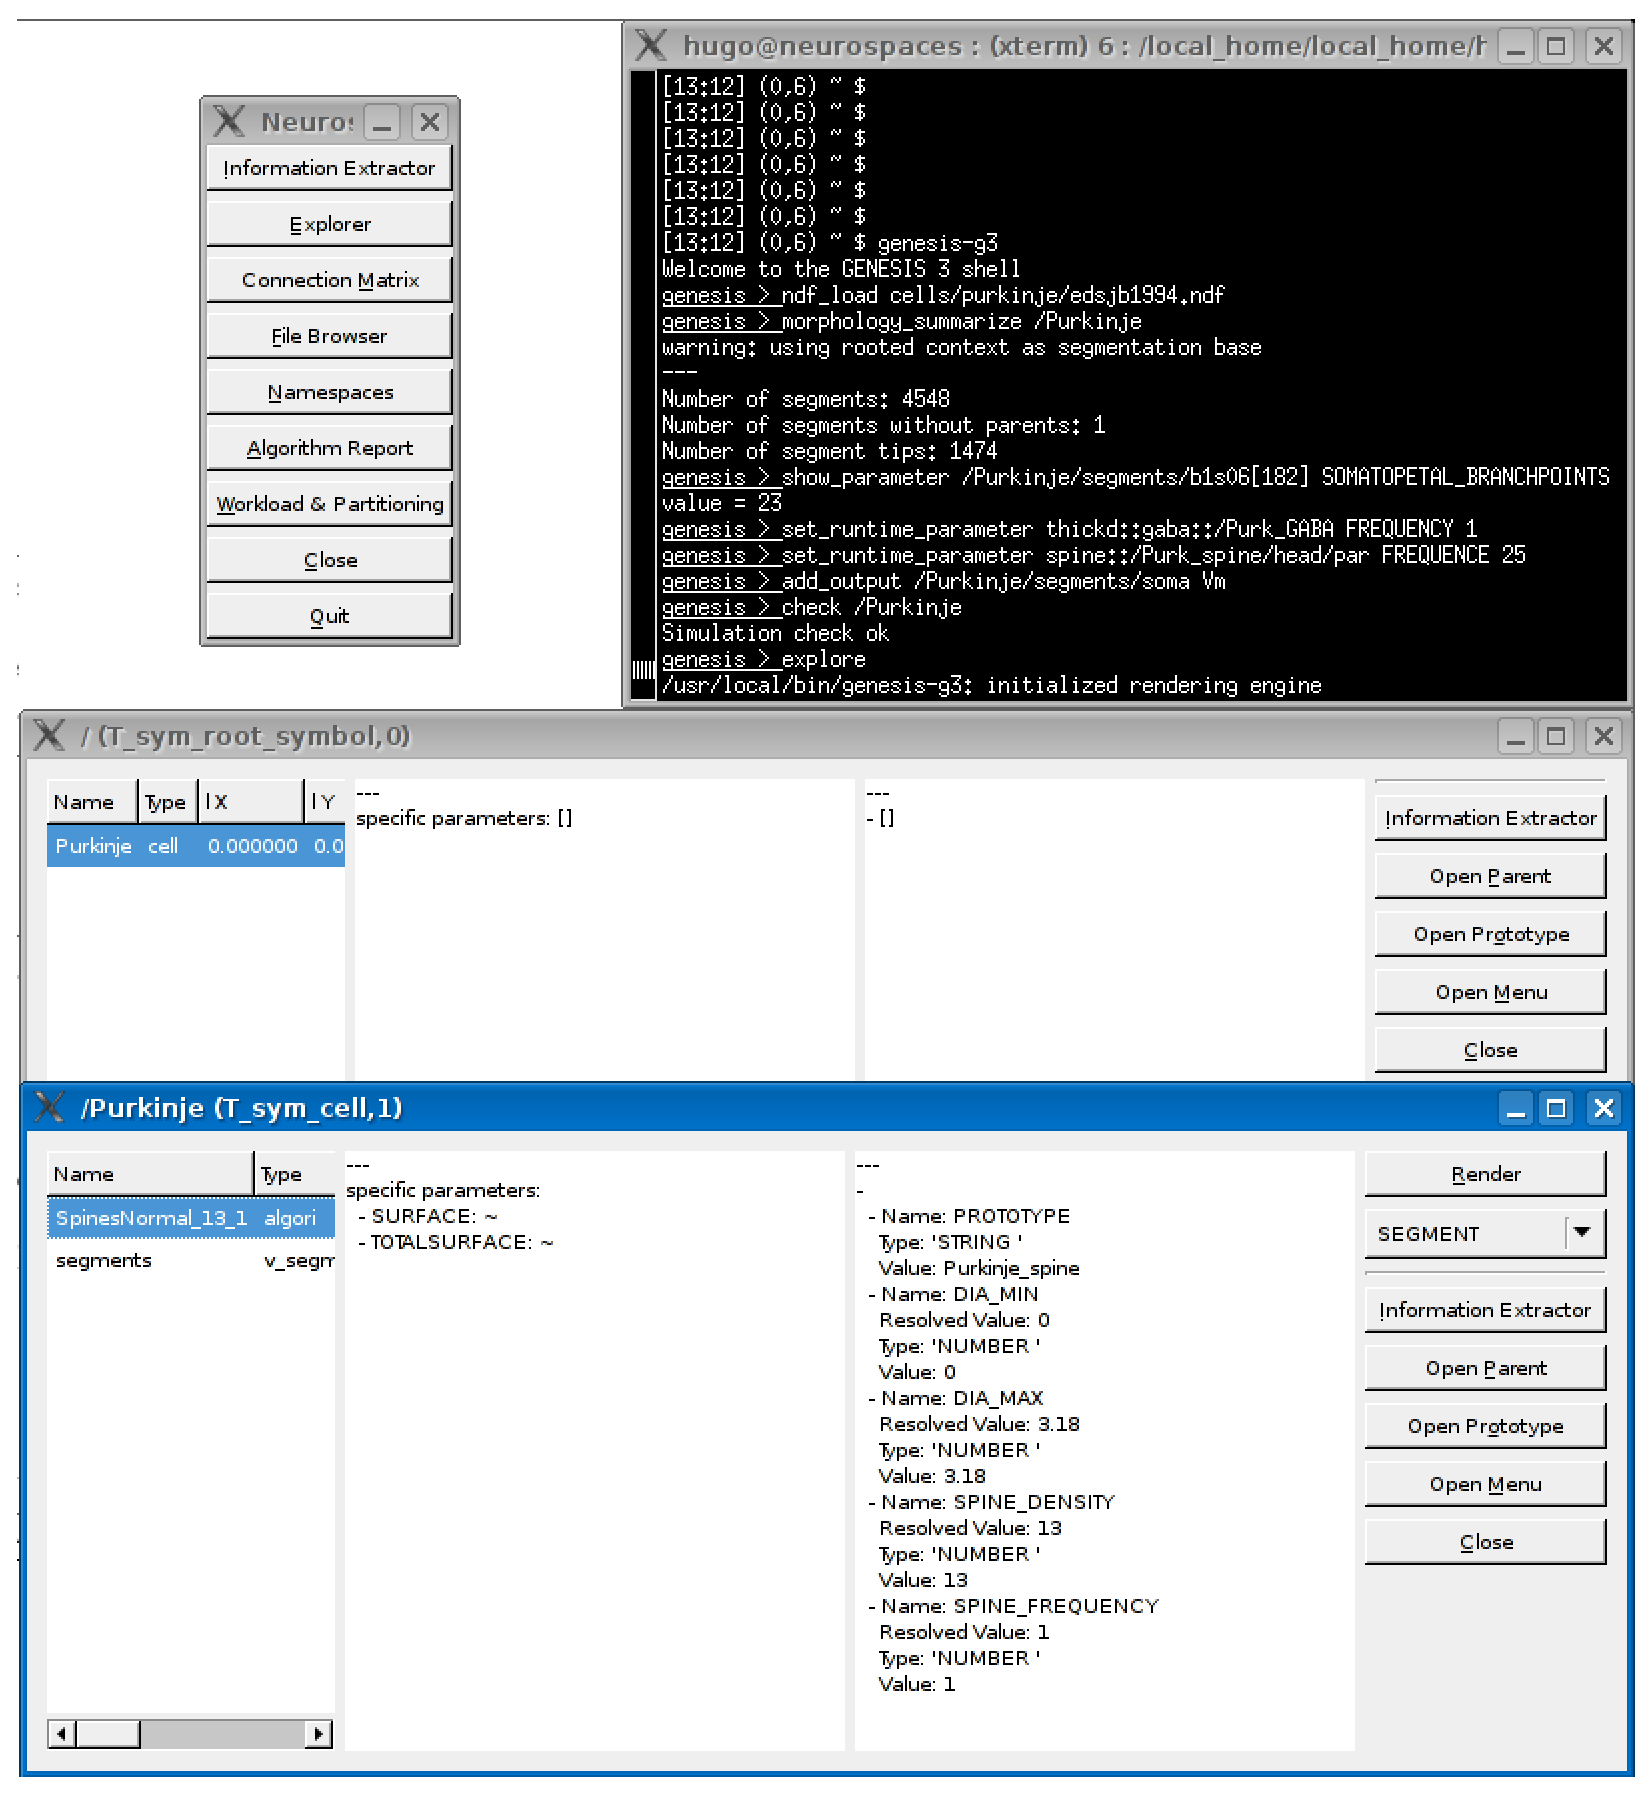
\includegraphics[width=0.45\textwidth]{figures/studio-screenshot.eps}
  \end{center}
  \caption{ \small{{\bf Querying a model in GENESIS 3.0.} The {\bf Studio} is a G-3 simulator component that can be used to query the parameters of individual compartments in a multi-compartment model neuron. The {\bf Studio} also renders 3D morphology of dendrites and generates overviews of network models.
  }}
  \label{fig:cbi-studio}
\end{figure}

Figure~\ref{fig:cbi-studio} shows sample output of running this command.  Other capabilities of the {\bf Studio} include rendering morphologies in three dimensions and generating overviews of network models (not shown). 

%In the next section we explore some of the more
%graphical capabilities of G-3.

\subsection{Simple Scripting}
\label{ss-apens}

Python is a high-level scripting language that uses modules to group related functions.  G-3 employs Python's module system to group the functions that provide an interface to each of the simulator's software components.
%G-3 scripting
%bindings use modules to separate interfaces for simple models with
%many default settings (e.g. to start a new research project) from more
%complicated interfaces that expose the full functionality of the
%simulator.
As an example, the G-3 Python module {\it nmc} contains functions to simplify the storage of neuron models in computer memory.  The module is a simple front-end to the {\bf Biology\,Model\,Container}. Likewise, {\it Heccer} is a wrapper module for the {\bf Heccer} component.  We note that Python bindings for {\bf DES} to facilitate network modelling are in development.

%Here we show a simple example of a high-level Python script that runs a simulation of a single cylindrical segment. It
%is defined by standard values for the parameters of membrane
%resistance ({\tt RM}), axial resistance ({\tt RA}), and membrane
%capacitance ({\tt CM}). (Note: This script
%  is written for clarity of presentation rather than compactness or
%  efficiency.)
%%\footnote{The solver requires {\tt RA} for all
%%  compartments.}
%Parameters are given by their specific values (in SI units) as
%commonly reported in the literature, instead of their actual values
%scaled to the compartment surface area as used by a mathematical
%solver \cite{cornelis04:_neuros_param_handl}. The script defines a
%Python function {\it run\_simulation} that will load and run a model when invoked from
%a system command line on an appropriately configured computer.  The script
%can also be imported into G-3 as a Python module, thus allowing access
%to this function.  For convenience, we call this Python module {\it
%  example}.
%
%\begin{verbatim}
%"""
%Comment: Python script running a simple model with G-3.
%"""
%from g3.nmc import ModelContainer
%
%def RunSimulation(simulationTime):
%    timeStep = 1e-5
%    
%#------------------------------------------------------------------------------
%# Create a model container with a neuron cell and a dendritic segment
%#------------------------------------------------------------------------------
%    my_nmc = ModelContainer()
%    my_cell = my_nmc.CreateCell("/cell")
%    my_segment = my_nmc.CreateSegment("/cell/soma")
%
%    my_segment.SetParameters(
%        {
%        "Vm_init": -0.0680,
%        "RM": 1.000,
%        "RA": 2.50,
%        "CM": 0.0164,
%        "ELEAK": -0.0800,
%        "DIA": 2e-05,
%        "LENGTH": 4.47e-05,
%        }
%        )
%
%# Apply current injection to the soma
%    my_segment.SetParameter("INJECT", 1e-9)
%
%#------------------------------------------------------------------------------
%# Create a Heccer for computing the neuron model stored by the model container.
%#------------------------------------------------------------------------------
%    from g3.heccer import Heccer
%    my_heccer = Heccer(name="/cell", model=my_nmc)
%    my_heccer.CompileAll()
%
%#----------------------------------------------------------------------------- 
%# Create an output object.
%#------------------------------------------------------------------------------
%    from g3.experiment.output import Output
%    my_output = Output("/tmp/output")
%
%#----------------------------------------------------------------------------- 
%# Link the output object to the address of the computed variable of interest.
%#------------------------------------------------------------------------------
%    my_output.AddOutput("output", my_heccer.GetAddress("/cell/soma", "Vm"))
%
%#----------------------------------------------------------------------------- 
%# Create an array of the objects that participate in the simulation.
%#------------------------------------------------------------------------------
%    schedulees = []
%
%    # schedule heccer
%    schedulees.append(my_heccer)
%    schedulees.append(my_output)
%
%#----------------------------------------------------------------------------- 
%# Advance all the particpating objects for the duration of the simulation.
%#------------------------------------------------------------------------------
%    currentTime = 0.0
%    while currentTime < simulationTime:
%        currentTime += timeStep
%
%        for schedulee in schedulees:
%            schedulee.Advance(currentTime)
%
%    my_heccer.Finish()
%    my_output.Finish()
%  
%#------------------------------------------------------------------------------
%# Main program executes a simulation of 0.5 seconds.
%# The if statement allows use of this file as an executable or as a library.
%#------------------------------------------------------------------------------
%
%if __name__ == '__main__':
%    RunSimulation(0.5)
%\end{verbatim}
%
%%# Second Example: use a wildcard to activate endogenous synapses (see text)
%%#    my_nmc.Query("setparameter spine::/Purk_spine/head/par 25")
%%#    my_nmc.Query("setparameter thickd::gaba::/Purk_GABA 1")

\subsection{Scripting Chemesis-3}

The following example, {\it cal1.ndf}, shows how to implement a G-2 Chemesis tutorial in G-3.  It creates a single compartment that contains interaction between calcium and a buffer.

%, {\it cal2.g} creates a two
%compartment model with a dendrite and soma with an additional diffusion object
%for diffusion between the compartments

\begin{tiny}
\begin{verbatim}
NEUROSPACES NDF
PUBLIC_MODELS
  KINETICS cal1
    PARAMETERS
      PARAMETER ( DIA = 24e-4 ),
      PARAMETER ( LENGTH = 24e-4 ),
    END PARAMETERS
    POOL somaCa
      BINDABLES OUTPUT concen END BINDABLES
      PARAMETERS
        PARAMETER ( concen_init = 0.001 ),
        PARAMETER ( "UNITS" = 1e-3 ),
      END PARAMETERS
    END POOL
    POOL somaCabuf
      BINDABLES OUTPUT concen END BINDABLES
      PARAMETERS
        PARAMETER ( concen_init = 0.003 ),
        PARAMETER ( "UNITS" = 1e-3 ),
      END PARAMETERS
    END POOL
    POOL somabuf
      BINDABLES OUTPUT concen END BINDABLES
      BINDINGS
        INPUT ../somaCabuf->concen,
      END BINDINGS
      PARAMETERS
        PARAMETER ( concen_init = 0.153 ),
        PARAMETER ( concen_total = 0.153 ),
      END PARAMETERS
    END POOL
    REACTION somacabufrxn
      BINDABLES INPUT concen, OUTPUT concen END BINDABLES
      BINDINGS
        INPUT ("substrate") ../somaCa->concen,
        INPUT ("substrate") ../somabuf->concen,
        INPUT ("product") ../somaCabuf->concen,
      END BINDINGS
      PARAMETERS
        PARAMETER ( FORWARD_RATE = 1e2 ),
        PARAMETER ( BACKWARD_RATE = 0.5 ),
      END PARAMETERS
    END REACTION
  END KINETICS
END PUBLIC_MODELS
\end{verbatim}
\end{tiny}

The length and diameter of the pools required to complete the model take on their implicit default values of:

\begin{tiny}
\begin{verbatim}
  PARAMETER ( DIA =  ..->DIA ),
  PARAMETER ( LENGTH =  ..->LENGTH ),
\end{verbatim}
\end{tiny}

The following commands illustrate how the {\bf G-Shell} and the {\bf Studio} may be employed to load  {\it cal1.ndf} into the {\bf Biology\,Model\,Container} for exploration of this model:

\begin{tiny}
\begin{verbatim}
  ndf_load chemesis/cal1.ndf
  explore
\end{verbatim}
\end{tiny}

%while, the {\bf G-Shell} command to run {\it cal1.ndf} and send output to
%a file is:
%
%\begin{verbatim}
%  genesis > run /cal1 2
%\end{verbatim}

\section{Results}

\subsection{Addressing Scheme Algorithm}

The different solvers contributing to a multiscale simulation can hold equivalent variables.  These variables exist because two or more physical processes of the model have been bound using the {\tt BINDINGS} in an NDF file.  During a simulation, {\it the addressing scheme algorithm} enables the {\bf Solvers} and the {\bf Communication\,Infrastructure} to relate any equivalent variables these components contain.  As this happens during a simulation, {\it the addressing scheme algorithm} must be highly optimized to maximize run-time performance.

The information required to identify a variable (and hence its address) is obtained from the model stored in the {\bf Biology\,Model\,Container}. To achieve this, the {\bf Biology\,Model\,Container} defines an addressing scheme that is able to refer to or `address' the variables of every model component. These addresses provide the `hooks' for attaching ``experimental protocols'' (e.g. stimulus and output specifications) to the {\bf Solvers}.  The addressing scheme is not necessarily dependent on the NDF format. It is more general in the sense that it provides an interface to external software applications such as GUIs and databases.

In G-3, the algorithm for taking the simulation-time address of a computed variable consists of three steps.

\paragraph{Step 1} Translates NDF names to a hierarchical namespace. The scheme defines a symbolic syntax for the hierarchical addressing of model components and their parameters and variables.  The syntax allows a user to express the address of a variable, for example, the address of the $\mathrm{Ca}^{2+}$ concentration in a segment, with the name `soma':

\begin{tiny}
\begin{verbatim}
  /soma/Ca->conc
\end{verbatim}
\end{tiny}

\paragraph{Step 2} The second step is the translation of symbolic references to IDs and is implemented in the {\bf  Biology\,Model\,Container}. There, the hierarchical namespace (created during step 1) is translated to simulation wide unique tuples of the form [integer, type].  The integer identifies the physical process and the type identifies the variable containing the concentration level.

%This constructs an interface that identifies the solver instance
%associated with each physical process (here the $\mathrm{Ca}^{2+}$
%pool).

%This translation is only required during simulation construction, and
%not during simulation run-time.  Once constructed, the tuples are
%independent of the {\bf Biology\,Model\,Container}.

\paragraph{Step 3} The third step of the addressing algorithm translates [integer, type] tuples to tuples of the form [solver instance, internal ID].  This step is low-level and implemented in the {\bf Solvers}.

After this step of the algorithm, an interface has been defined that enables the communication port of the solver that attaches to the given variables to be obtained.  This interface allows a solver instance internal ID to be obtained for directly addressing the variable.

The addressing scheme algorithm allows {\bf Solvers} to communicate through the tuples [solver instance, internal ID].  The advantage is that the {\bf Biology\,Model\,Container} does not have to be in memory during simulation run-time.  This removes any requirement for expensive computation on symbolic or hierarchical addresses during simulation run-time.

Software may choose to implement the interface between solvers using memory pointers for maximum efficiency, or, alternatively, using a low-level function that reads and writes the variable.  This feature may be useful in a parallel implementation for example.

%  However it may be required during
%simulation run-time, depending on the model and stimulus
%paradigm\marginpar{I don't see when?}.


\subsection{DES: Action Potential Propagation Abstraction}

The Discrete Event System ({\bf DES}) is used for the abstract modelling of action potentials, a functionality required for the running of network simulations.  Action potentials generated at the soma of one neuron are translated to a discrete event that is delivered to the post-synaptic targets of a connected neuron.  {\bf  DES} also associates `secondary' data with a connection, for example, propagation delay, synaptic weight, or other data specific for the model.

Internally, {\bf DES} contains two subcomponents, one for event distribution that contains a connectivity matrix, the second for event queuing.  In the CBI architecture, the {\bf DES} event queuer is a separate solver that simulates action potential propagation in an efficient way.  The {\bf DES} event distributor provides communication between the solvers during the simulation.

The separation of the discrete event functionality from the rest of the simulator facilitates customization for the modeling of sophisticated learning rules, especially those related to STDP, diffusion, and spillover \cite{roberts02:_spike, nowotny03:_enhan}.

\subsection{Multiscale Network Modeling}

Network modelling was previously possible in G-2 \cite{cornelis02:_tutor}.  To simulate networks of cells the user must manually initialize the numerical solver of G-2 for every cell in the network.  Careful G-2 script coding was required to prevent memory exhaustion errors.  The complexity of the G-2 procedural scripts contrasts with the simplicity of the configuration of the G-3 addressing scheme given below.

The {\bf SSP} software component defines several software regression tests with network models.  One of the simplest network models used in
this test has a `source' neuron that delivers a spike to two `target' neurons during the simulation .

To simulate this simple network, the simulation configuration has to associate each neuron model in the {\bf Model\,Container} with {\bf   Heccer}.  This association will then create a {\bf Heccer} instance before the simulation starts.  As with G-2, in G-3 this is currently a manual operation.
%In G-3 multiscale network modelling of individual neurons requires a
%{\bf Heccer} instance for each neuron.
However, the integration of the user workflow into G-3 defines the scope of user actions and in the case of network modeling, allows the {\bf Heccer} instances, once created, to share internal data structures as required, thereby transparently reducing overall memory consumption.

In G-3 the action potential propagation through the fibers of a projection is simulated by the event queuing component of {\bf DES}. The {\bf G-Shell} syntax is:

\begin{tiny}
\begin{verbatim}
  ndf_load tests/networks/spiker4.ndf
  solverset "/network/target1 => heccer"
  solverset "/network/target2 => heccer"
  solverset "/network/source => heccer"
  solverset "/network/projection => des"
\end{verbatim}
\end{tiny}
%Internally, the {\bf G-Shell} translates these statements to their
%equivalent {\bf SSP} syntax:
%\begin{verbatim}
%  { modelname => "/network/target1",
%    solverclass => "heccer", },
%  { modelname => "/network/target2",
%    solverclass => "heccer", },
%  { modelname => "/network/source",
%    solverclass => "heccer", },
%  { modelname => "/network/projection1",
%    solverclass => "des", },
%\end{verbatim}

\subsection{Multiscale Scripting}

In  a typical multiscale model different numerical solution methods are required to solve the different types of mathematical equations associated with the different scales of the model.  In G-3 the cable equation and ion currents are numerically solved with implicit Crank-Nicolson integration using {\bf Heccer}.  Calcium models are numerically solved with {\bf Chemesis-3}. The association between a given model and its {\bf Solvers} can be configured by the user.
%Under planned extensions to the G-shell syntax, the correct syntax
%for a loaded single neuron model with name "/Purkinje" would be:
For example to associate the model named ``/Purkinje'' with the solver {\bf heccer}, the command is:

\begin{tiny}
\begin{verbatim}
  solverset "/Purkinje => heccer"
\end{verbatim}
\end{tiny}

To use {\bf Chemesis-3} to simulate a complex network model of biochemical pathways, here called {\it cal1}, a user would type in the G-3 shell:

\begin{tiny}
\begin{verbatim}
  solverset "/cal1 => chemesis3"
\end{verbatim}
\end{tiny}

In the case where a network of biochemical pathways is defined inside a single neuron model, a user would have to type two commands with wildcards to associate the correct solver with each component of the model, for example:

\begin{tiny}
\begin{verbatim}
  solverset "/**/cal1 => chemesis3"
  solverset "/Purkinje/**[!cal1] => heccer"
\end{verbatim}
\end{tiny}

%In later versions of G-3 these rules will be built in but still allow
%the user to select a different method of solution for different
%components of a model.

\section{Discussion}

The papers reflect the cognitive process of the investigators doing the work.

\subsection{The Celestial Hierarchy and Great Chain of Being}
The multiscale problem, at its origin, started with the idea of {\it The Great Chain of Being}. {\it The Great Chain of Being} is a hierarchical structure of all matter and life, thought by medieval Christianity to have been decreed by God. It begins with God and descends through angels, humans, animals and plants to minerals. The idea extended across more than two millennia and together with its axiomatic principles of, ``plenitude,' ``continuity'', and ``graduation," from the time of Plato was one of the most famous in the vocabulary of Western theology, philosophy, and science~\citep{lovejoy48}. Until about the 1850s, it was probably the most widely familiar conception of the general scheme of things and of the constitutive patterns of the universe. One hundred years later, in the middle of the twentieth century, it was recognised as a concept that had become one of the half-dozen most potent and persistent presuppositions in Western thought.

The idea of a hierarchical chain of levels can be seen as an example par excellence of a simplifying organizational principle whereby to understand cerebral cytoarchitecture, i.e. the cognitive model, but also provides an organizational framework that enables understanding thus principled model implementation based on hierarchical frameworks encapsulating levels of organization and function associated with the neural structures observed within the anatomy of the mammalian central nervous system. The approach seems necessarily to continue to predetermine and drive much ongoing theory and many ideas considered fundamental concerning the understanding of nervous system function.

\subsection{The Multiscale Problem}
While seeming both transparent and widely accepted, some authors consider a careful definition of the term multiscale should be identified as it is a recent notion that very quickly spirals into a realm of catch-all scientific jargon~\citep[for example][]{walpole13}. That such freedom is encouraged is evidenced by the absence of the term from \textit{The Encyclopedia of Computational Neuroscience}~\citep{jung22}, where nine years after its initial publication there is neither section nor article devoted to the difficulties of multiscale computation. More trivially, the term appears on ten occasions in the 3,663 pages of the second edition and also in a total of twelve publication titles cited in the References that follow each entry in the Encyclopedia.

Historically, multiscale modelling has primarily been explored in the fields of engineering, computer sciences, and physics, where multiple scales of observation have motivated extensive use of this approach. More recently, computational neuroscience has shown an increased interest in this discipline. It is now recognised as being essential for a better understanding of nervous systems and how molecular level neuronal events modify underlying neural circuits and brain function, thus both innate and learned behaviours~\citep{bouteiller11}.

Founded on the widely accepted paradigm exemplified in Figure~\ref{fig:multi-scale-taxonomy} that the central nervous system is a highly hierarchical structure that integrates several spatial and temporal levels of complexity~\citep{bouteiller11}, the concept of multiscale modelling has been implemented by employing different models, possibly described by different physical formalisms and acting simultaneously on different temporal and spatial scales, so as to study important features of complex phenomena at multiple levels of organization~\citep{djurfeldt07}.

Thus, a multiscale model typically accounts for more than one magnitude of resolution across discriminable functional domains~\citep{walpole13}. However, many models of physical systems implicitly account for multiple resolutions by simplifying their boundary conditions\marginpar{\scriptsize Needs one sentence more explanation?} into “black boxes” where assumptions about other spatial or temporal domains are summarized by governing equations. Further, explicitly modeled tiers of resolution must also provide additional information unobtainable by independent exploration at a single resolution. This latter requirement is one that enables a fundamentally important distinction to be made between explanatory models and mere demonstrations. Notably, in a similar way, respectively, a theory provides an explanation, whereas, a law provides a description~\citep{schurger22}.

\subsection{Evolution of the Classical Neuroscientific View -- continued}

One consequence of this preference was emergence of a doctrine that emphasised top-down as opposed to bottom-up investigation and modelling as the neurobiological facts were only a matter of implementation.

Briefly, top-down investigation relies on estimation of mean behavior at a macroscopic level; thus modeling populations, not single entities~\citep{chiacchio14}. It proceeds by use of ordinary and partial differential (ODE and PDE) equations. ODE-based models tend to ignore topology, whereas PDEs can be used when spatial dimensions are of interest. However, both techniques ignore individual interactions.

Alternatively, in a bottom-up approach interactions are described and followed individually. The general behavior of the system arises from the sum of the local behaviors, local activity is described with greater accuracy and approximations typical of a top-down approach are avoided. Furthermore, spatial distribution and stochastic behaviors are intrinsic features normally represented by this technique. However, as entities are followed individually, greater computational effort is required and there are no strong mathematical instruments available for analytical study~\citep{chiacchio14}.

Such schemas are typically embedded in a framework that knowingly or otherwise espouses a practice of divide and conquer where smaller and smaller parts and/or components are studied in the expectation that the whole can be understood through a divisive principle referred to as hierarchical reductionism~\citep{dawkins06}. This is despite the fact that it remains uncertain as to whether the brain can be understood as the interaction between independently describable subsystems~\citep{djurfeldt08}. Although, a recent report that started from the molecular level in a bottom-up approach that integrated molecular events into synaptic and neuronal architectures seems to provide convincing evidence that this may not actually be possible~\citep{bouteiller11}.

Alternatively, ~\citet{bojak22} has proposed that within a decade or two, top-down neural population models will take their rightful place as the primary means by which mesoscopic brain activity is described. It is claimed further that the central problem to be faced by bottom-up descriptions is not the simulation of millions of neurons in a reasonable amount of time, but rather that the properties and interactions of that number of neurons cannot be specified in a biologically meaningful manner and cannot generate actual human insight into principles of function from the plethora of individual cell activities. Rather, progress is to be made via multiscale descriptions wherein higher levels discard the irrelevant detail of lower levels to facilitate effective and efficient models that remain accessible to the human mind. Further, it is expected that in the future, given their intimate connection to (noninvasive) neuroimaging, such neural population models will play a privileged role.

Thus, for the foregoing reasons, amongst others canvassed here, the metaphors employed to provide the framework for the cognitive models subserving neuroscience in general and computational neuroscience in particular, must be chosen with great care.

Ultimately, however, computational neuroscience is proposed to offer multiscale models that span complexity from the level of the gene to the whole living system, spanning different temporal and spatial scales~\citep{jung22}.

\subsection{So, What Is Scientific?}

When initiating a new project it is often of value to explore the meaning and origins of the semantics within which it is buried. Here, the interest lies in elucidation of a framework that enables what is referred to as scale-independent neural simulation.

For more than 1,500 years anatomical and physical ideas concerning the structure and function of the human nervous system settled into an enduring dogma that encompassed the time of Galen ({\small{AD}}\,129--199) in antiquity to that of Haller ({\small{AD}}\,1708--1777) in the eighteenth century~\citep{clarke87}. It subsequently disappeared during the first half of the nineteenth century as a scientific revolution ushered in a new understanding of the nervous system. Outmoded ideas were displaced by fundamental new neuroscientific concepts of the nervous system that were developed, became established during that half century, and subsequently have survived in modified form into the twenty-first century. In short, it is not unreasonable to consider that by 1850, with the exception of the idea of localization of function in the brain, the foundations of modern experimental neuroscience had been laid.

Deeply influenced by the philosophical thought of that time, an otherwise inexplicable change in the experimentalist's attitude to brain activity could be attributed to investigators such as Flourens on the basis of his claim that in experimental research everything depends on the method~\citep{flourens24}.

Technology, however sophisticated, is only one element of scientific creativity. The human element in science is primary. An investigator must frame meaningful questions, devise programs of research, and draw productive conclusions if there is to be any significant contribution to knowledge~\citep{clarke87}. Nowhere is this likely better demonstrated than with the identification of electricity with nervous activity by Galvani (1770)~\citet{galvani91} when he demonstrated muscle contraction in the frog leg after a wire in contact with a nerve fibre conducted an electrical spark. It then took almost 200 years via Nernst~\citet{nernst89} and Lapicque~\citet{lapicque07} before Hodgkin and Huxley~\citet{hodgkin52e} mathematically described the differential conductances in the membrane of a squid nerve fibre that underlay the generation of an action potential. It was with those experiments and their mathematical model that computational neuroscience came of age.

In one important way, many predictions in the biological sciences differ from those made in the physical sciences, particularly classical physics~\citep{darwin71}. In physics and engineering, most simple predictions or tests of hypotheses are deterministic. Whereas, in biology and particularly in neuroscience, many predictions where they can be made, are inherently probabilistic.

Simulation provides a framework to organize our understanding of biological systems. Historically, the development of neuronal simulation software for the construction of morphologically detailed neuron models and small networks has been instigated by research projects that specifically addressed complementary technical and scientific questions \cite{Moore:2010vn}. These software systems have been both highly successful and continue to grow in complexity through cycles of research project extension. However, after more than twenty years of extending their functionality, usually by the direct incorporation of source code into the core of the simulator (typically comprising a single solver), code structures have become so complicated that it is increasingly difficult, if not impossible, to easily continue extension of simulator functionality. Ultimately, the resulting stand-alone applications become `monolithic'. In these conditions it is a considerable challenge for a neuroscientist lacking the necessary mathematical and computational skills to extend a model. In practice, the complexity and monolithic nature of the software results in a non-scalable software architecture \cite{jaeger02:_comput_neuros_realis_model_exper}.

At the core of the problem is the lack of distinction in many contemporary simulators made between biological data, numerical data, and control operations during the software architecture development stage of simulator design. The majority of such simulators remain primarily focused on the biological and mathematical aspects of a model. As they do not respect all three of Marr's levels, i.e. the third of Marr's levels (``hardware'' implementation) is not addressed during software design, the complexity of multiscale simulation is greatly increased. 

We note that just as the `hardware' of a biological system should be accounted for in the cognitive process of model development, so must it be accounted for during the simulation of the model. In a simulator this can be achieved by the software architecture and its organization of simulator functionality. Making the cognitive model concordant with simulator functionality removes many of the problematic aspects of multiscale modeling.  

It has previously been proposed that \cite{Sejnowski:1988fk}: (1) because of the the many different structural levels of organization and the fact that models rarely span more than two levels, a more comprehensive understanding of a system requires many different types of model, and (2) intermediate level models must necessarily simplify with respect to the structural properties of lower level elements. We consider this view to be based on the difficulty of employing a monolithic simulator to address a multi-level problem.

To clarify these issues, we turn to a discussion in \cite{Heylighen:2006vn}. Systems theory shows that regardless of the number of scales used to conceptualize a system, it is not possible to know whether the system has been completely conceptualized. This is a consequence of changing scales as when this occurs it adds, deletes, and reconfigures patterns that are the content of the associated conceptualizations. There is no way to know or learn that all patterns have been conceptualized at one or more scales, as completeness is not possible. Nevertheless, the use of multiple scales of conceptualization provides a way to asymptotically approach completeness.
 
However, as \citet{Heylighen:2006vn} continues, at any scale of conceptualization, properties are always aggregated at least as simple objects. Thus, a system at any scale of conceptualization is an approximation or loose congruence of the actual system. This is not an `abstraction' of the system as that means leaving things out of a model with the understanding that what is absent can always be reinserted. What is ``left out'' of a scale specific conceptualization of a system are patterns (simple objects, relationships, and their aggregations) that might be available at other scales. Such patterns cannot be returned to a scale specific approximation of a system, regardless of resolution or field of view. This means that `missing' content has no place in a conceptualization at a given scale as it was never available in the first place.

According to principles of systems theoretic analysis (see \cite{Bertalanffy:1973zr,Heylighen:2006vn}), it is clear there are numerous phenomenological approaches to the development of multiscale models suited to the transformation of a mental model into a computational simulation. We resolve this problem by expansion of the cognitive workflow as illustrated in Figure \ref{fig:mental-model-simulation-path}.

The cognitive workflow is an adaption of a previously described user workflow that organizes the sequence of necessary steps typically employed by a person in developing a computational model and employing simulation to generate data for subsequent analysis \cite{cornelis12}. In this sense it is a depiction of a sequence of operations, declared as the work of a person or a group of persons (Belhajjame et al., 2002). Similarly, the cognitive workflow describes the process whereby an abstraction is transformed into an implementation by the conversion of a mental model into a simulation. This is made possible due to the recent reconfiguration of the GENESIS simulator. 

The reconfiguration complied with the CBI architecture which is based on a separation of concerns. It partitions data and control functions from software layering that separates high level biological data from low level mathematical operations. The immediate benefit of this partitioning (see \cite{cornelis12} for details), is transparent support of multiscale simulation.

The approach is based on the implementation of a model for simulation being contained by a single software entity (here a single {\bf Biology\,Model\,Container}). This single entity interfaces with the multiple solvers required to address the different scales of a model, but it is only needed during the construction of the model. A communication infrastructure enables communication at run-time between these solvers and thus across different levels of a simulation. In this paradigm, the requirement for multiple models is removed by implementation of multiple solvers. As a consequence, simplification of intermediate models with respect to lower levels as proposed by \cite{Sejnowski:1988fk} may be eliminated. 

%, but ought to attempt to incorporate as many of the given level's functional properties as actually exist in the higher level's computational tasks. This approach has led to the development of both realistic brain models containing considerable biological detail and simplifying brain models that `abstract' both structural and functional principles, although any given model may have features of both.

%The CBI architecture was designed to address this situation, thereby enabling transparent simulator extensibility and as a consequence the implicit implementation of multiscale modelling.

%The core of these problem is the 
%lack of distinction in the majority of contemporary simulators between biological data, numerical data, and control operations during the design and development of a simulator. The majority of contemporary simulators remain primarily focused on these biological and mathematical aspects of a model. As they do not respect all three of Marr's levels, the complexity of multiscale simulation is greatly increased. 

To this end, G-3 supports the construction of multiscale network and system models based on realistic neuronal components.  In support of
this function, the G-3 {\bf Biology\,Model\,Container} applies specific algorithms to instantiate systems level connectivity models and convert them to mathematical representations. This relieves the mathematical solvers from the algorithmic pressures typical for rich heterogeneous model structures.  At the same time, intermediate simulation system modules, already described as the mechanism used to link {\bf Chemesis-3} and linear cable solvers, are used to share values and functions between larger scale network simulations and lower scale models.

From a technical point of view, the incorporation of simulation modules that specifically involve spatial dimensions is, in principle, much more difficult than the integration of biochemical kinetic models. In fact the accurate representation of space and time for multiscale simulations is an open research area.  However, the explicit provision of software modules for the intermediary representation of solved variables allows the comparison and evaluation of different methods of scale-linking, for instance by comparing different resolutions of a fixed grid with adaptive grid intermediary
representations \cite{MO:2009bh}. In effect, this allows the use of multiscale G-3 models as a framework to compare different technical strategies.

A significant motivating factor for the work reported here was ably described by~\citet{sperry80} who noted that in attempting to understand brain physiology and function, at stake are central key concepts that directly involve fundamental convictions regarding the nature of man's inner being, physical reality, the meaning of existence, and related matters of ultimate concern, perspectives which in this area profoundly shape human value systems and societal decision-making and hence human destiny.

The developing paradigm of multiscale modelling reported here enables the generation of a taxonomy of models in computational neurobiology
based on both the biological scale of a model and the level of detail it aims to represent. By accounting for each of the levels proposed in \cite{Marr:1982fk} during development of a simulator, it is possible to transparently resolve many of the technical and conceptual issues currently surrounding the successful simulation of multiscale models.

%Ignoring these distinctions results in `collapse' of the cognitive workflow into a single node located at the last step of the cognitive workflow. This convergence is illustrated in Figure \ref{fig:mental-model-simulation-part}. The figure shows that in a monolithic software system high convergence allows only a single (monolithic) software component to exist. This suggests that in the absence of a clean separation of concerns, otherwise prohibited diagonal interactions are introduced between the Control/Data and High/Low software axes defined in Figure \ref{fig:cbi-architecture-simple}.
%
%\begin{figure}[h!t]
%  \begin{center}
%    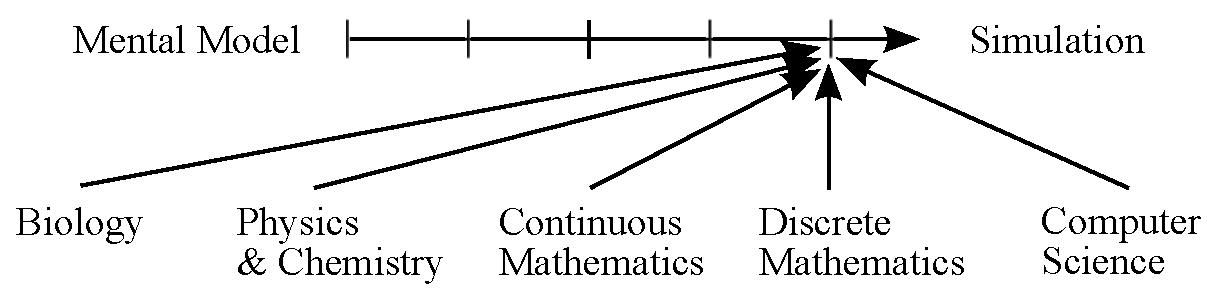
\includegraphics[width=4in]{figures/NS-abstraction-implementation-part.eps}
%  \end{center}
%  \caption{ {\bf Cognitive Workflow of Monolithic Software.} }
%  \label{fig:mental-model-simulation-part}
%\end{figure}
 
%Figure \ref{fig:mental-model-simulation-path} illustrates a selection of some of the possible steps, levels, and components of the cognitive workflow we employ here. Interestingly, two possible multiscale models have been in widespread use but not generally recognized for their multiscale characteristics: (1) Biologically inspired, e.g. a model is specified as a network and a population of detailed channel models, and (2) Mathematically inspired, e.g. use continuous cable equations to model a neuron, discrete event models for axonal propagation, and Hodgkin-Huxley equations for the channels.

 % Contrast this with \cite{ray08:_pymoos}

%- Summary.
%
%- Parts of the multiscale grant.

%\begin{figure}[ht]
%  \begin{center}
%    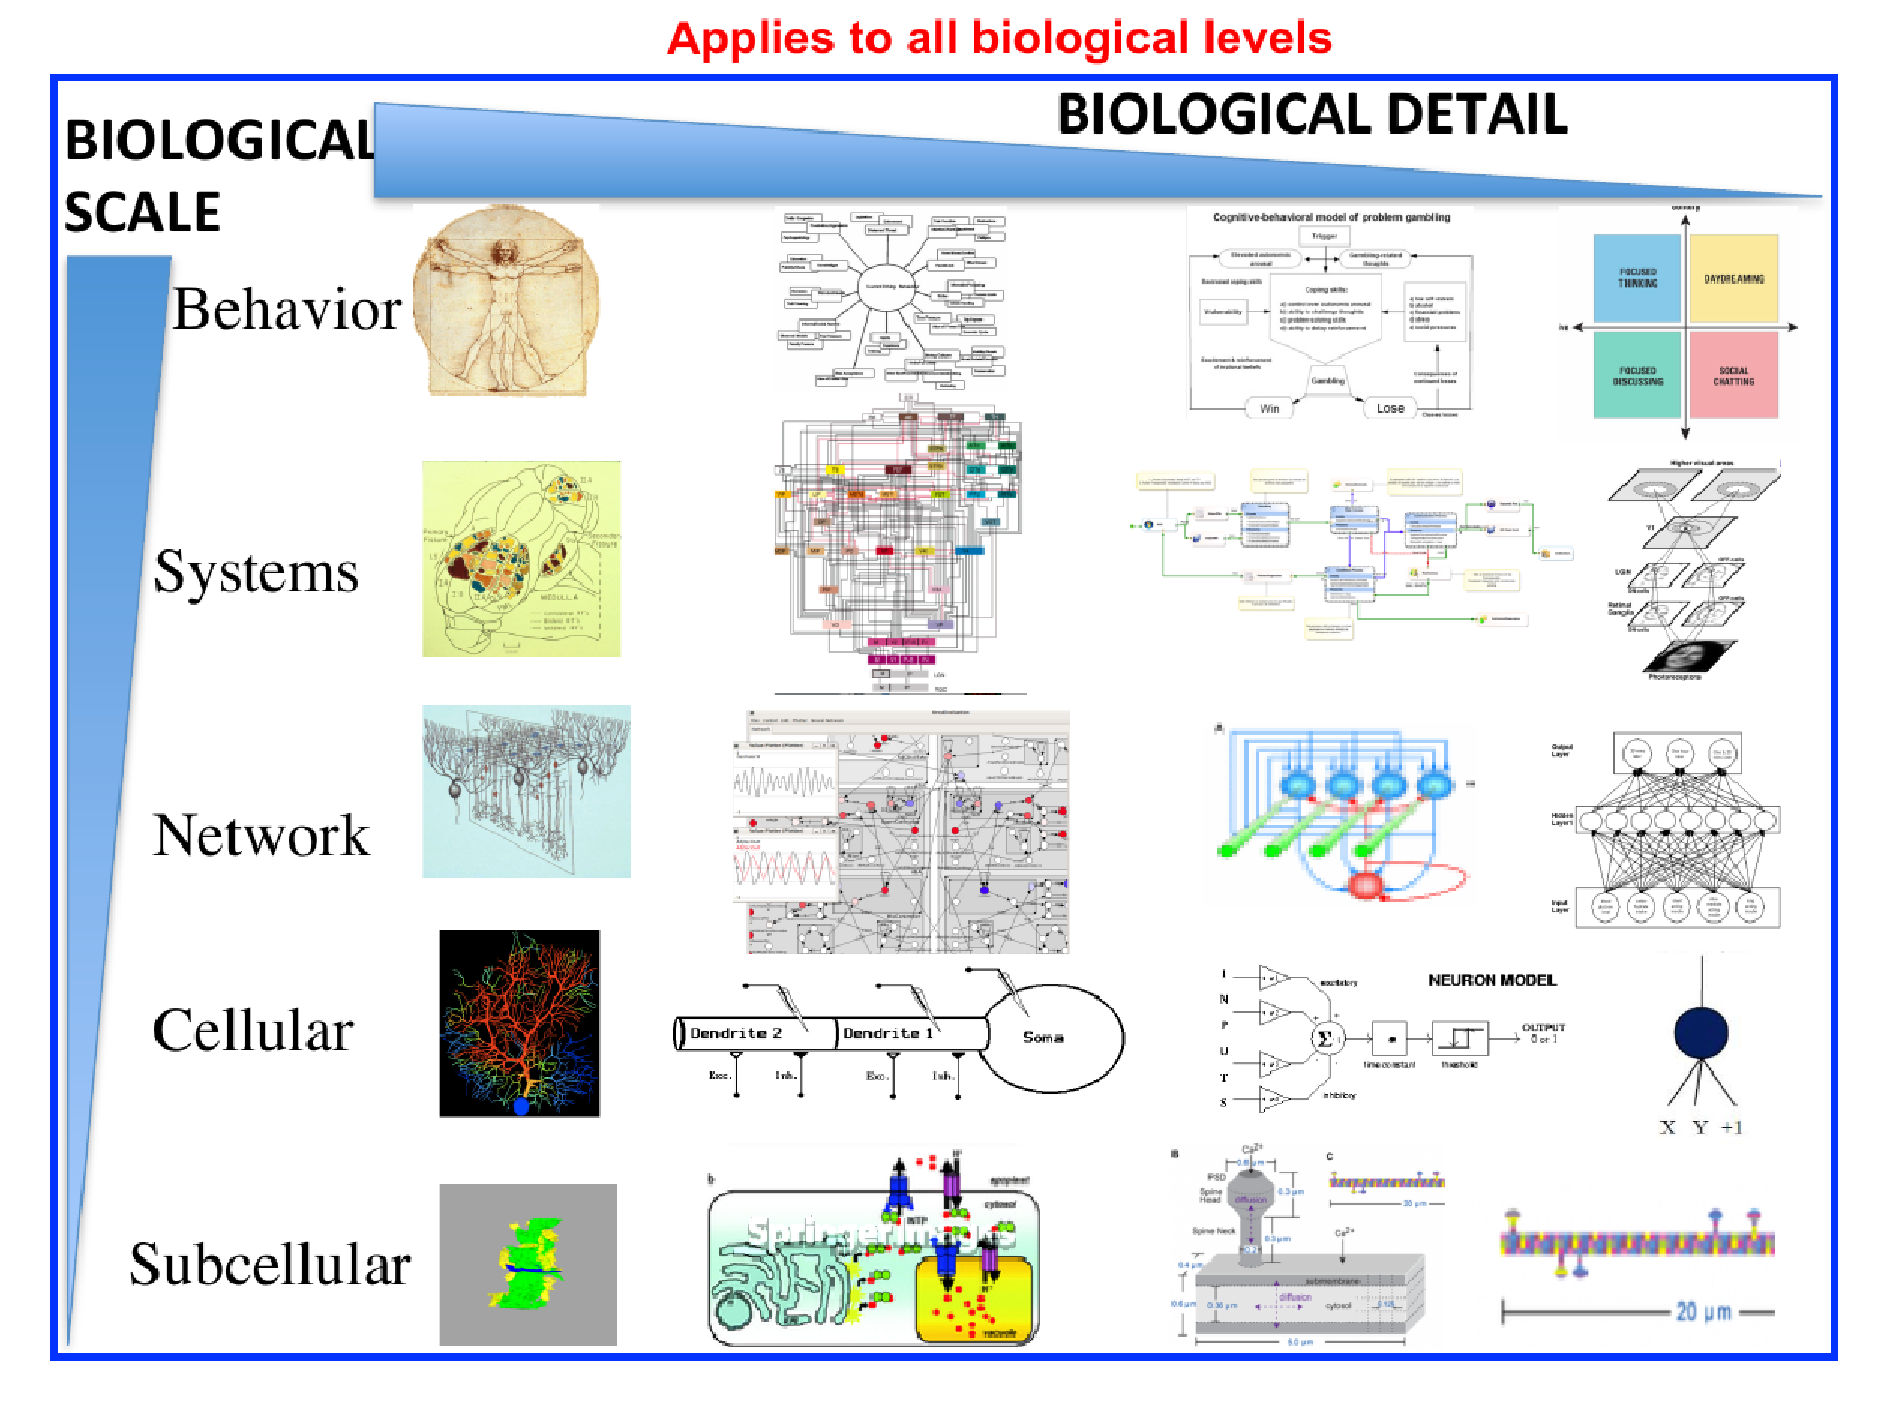
\includegraphics[width=4in]{figures/multi-scale-taxonomy.eps}
%  \end{center}
%  \caption{ {\bf Taxonomy of Multiscale Models.} }
%  \label{fig:multi-scale-taxonomy}
%\end{figure}

%Incorporate two types of 3-D Monte Carlo-based techniques for modeling
%reaction/diffusion kinetics. Specifically, Dr. Avrama Blackwell will
%work with the G-3 development team to implement NeuroRD (Oliveira et
%al., 2010), a computationally efficient approximate Monte Carlo
%approach to modeling reaction-diffusion systems.
%
%In addition, the G-3 development team will work with Dr. Yoshi Kubota
%to incorporate 'CDS' (Cellular Dynamics Simulator:
%http://nba.uth.tmc.edu/cds/) a precise particle-based Monte Carlo
%simulator specifically supporting the modeling of Ca2+ binding and
%diffusion dynamics within biochemical networks (Byrne et al. 2010;
%Kubota and Waxham 2011). CDS is based on the event-driven first
%passage time algorithm (Byrne et al. 2010) and is designed to serve as
%a flexible platform for multiscale hybrid algorithms.  For this
%reason, the CDS algorithm can be directly combined with any
%deterministic ODE/PDE (Reaction-Diffusion Equation) solvers (e.g.,
%V-Cell used in Hernjak et al. 2005) including those already included
%in G-3.  High-resolution cellular morphology including that of
%dendritic spines can be directly transported to CDS allowing
%electro-diffusion to be simulated by both deterministic (as in
%Lopreore et al. 2008) as well as particle-based 3-D stochastic
%methods.
%
%This will allow us to compare different simulation algorithms for Ca2+
%binding diffusion, voltage clamp, and biochemical network within the
%same platform and will help derive and validate simplified macroscopic
%(biochemical) synaptic rules relevant to the objectives of Specific
%Aim 2.

%\subsection{additional references}
%
%DeSchutter, E., and Bower, J.M. (1994)  An Active Membrane Model of the
%Cerebellar Purkinje Cell: I simulation of current clamps in slice   J.
%Neurophysiol.  71:375-400.
%
%Kotaleski, J. H., Plenz, D. and Blackwell, K. T. (2006) Using potassium
%currents to solve signal-to-noise problems in inhibitory feedforward
%networks of the striatum. J. Neurophysiol.  95: 331-341.
%
%- dave's chapter
%
%- visual interface to neuron (see Jim's review invitation)
%
%- numerical solvers, see Andrew Davison's email.

\section*{Acknowledgements}

Hugo Cornelis is an embedded software engineer contracted with Essensium NV, Leuven, Belgium, EU.\\
Allan D. Coop commends the Australian and United States Federal Governments for their support of employable people through a Universal Basic Wage.


\section{Conflict of Interest Statement}

The authors declare no conflict of interest.

%%\textbf{Citation and Referencing}

\bibliography{../tex/bib/2023-07-21-g3-refs-adc-1}

\end{document}

